\documentclass[12pt,a4paper,twoside]{report}
\usepackage[utf8]{inputenc}
\usepackage{amsmath}
\usepackage{amsfonts}
\usepackage{amssymb}
\author{Edward Seabrook} 
\title{Third Year Project Final Report}

\usepackage{nomencl}
\makenomenclature

%Might be useful if I cut about 4 entires
%\setlength{\nomitemsep}{-\parsep}

% Makes Chapter heading look like Section heading
\usepackage{titlesec}
\titleformat{\chapter}% reformat chapter headings
    [hang]% like section, with number on same line
    {\Large\bfseries}% formatting applied to whole
    {\thechapter}% Chapter number
    {0.5em}% space between # and title
    {}% formatting applied just to title

% Save a bit of space by giving all headings less room
\titlespacing*{\chapter}{0pt}{0pt}{0pt}
\titlespacing*{\section}{0pt}{0pt}{5pt}
\titlespacing*{\subsection}{0pt}{0pt}{5pt}
\titlespacing*{\subsubsection}{0pt}{0pt}{5pt}
\titlespacing*{\paragraph}{0pt}{0pt}{5pt}

\widowpenalty=10000
\clubpenalty=10000

% Set margins to required
\usepackage[top=2.4cm, bottom=2.4cm, left=2.95cm, right=2.95cm]{geometry} 

% Sort out margins for todonotes
\setlength{\marginparwidth}{3cm}
\reversemarginpar

\renewcommand*\ttdefault{cmtt}
\usepackage[T1]{fontenc}

\usepackage{listings}
\lstset{basicstyle=\ttfamily, escapechar=\%}

\newcommand*{\mysym}{\mathord{\sim}}

% Set paragraph spacing to required
\setlength\parindent{0pt}
\usepackage[parfill]{parskip}

\usepackage{hyperref}
\usepackage{todonotes}
\usepackage{listings}
\usepackage{appendix}
\usepackage{pdflscape}
\usepackage{cite}
\usepackage{wrapfig}

\hypersetup{colorlinks=false, pdfborder={0 0 0}, }

% Not totally sure
\usepackage{fancyhdr} 
\pagestyle{fancy} 
\renewcommand{\headrulewidth}{0pt} 
\lhead{}\chead{}\rhead{}
\lfoot{}\cfoot{\thepage}\rfoot{}

% Number and show in ToC to a deeper level
\setcounter{secnumdepth}{3}
\setcounter{tocdepth}{3}

\def\nomlabel#1{\textbf{#1}\hfil}

\begin{document}

% Include title page

\begin{titlepage}

\begin{center}


% Upper part of the page
%\includegraphics[width=0.15\textwidth]{./logo}\\[1cm]    

\LARGE Electronics and Computer Science\\
Faculty of Physical and Applied Sciences\\
University of Southampton
\\[1.5cm]

\href{mailto:ejfs1g10@ecs.soton.ac.uk}{Edward JF Seabrook}\\[0.5cm]

\today \\[1cm]
{\bfseries A Tool to Simplify Network Administration in the Modern Home}\\[1.5cm]

\vfill

% Author and supervisor
\large
Project Supervisor: 
Dr.~T \textsc{Chown}\\

\large
Secondary Examiner:
Dr.~KP \textsc{Zauner} 

\vfill

A Project Progress Report Submitted for the Award of Computer Science

\end{center}

\end{titlepage}


\begin{abstract}
As the complexity of home networks increases, it is inevitable that they will
require splitting into multiple subnets. As the average home user is unable to
configure a router, a minimal configuration solution is required. In this
project I made enhancements to an existing implementation of the Open Shortest
Path First for IPv6 (OSPFv3) routing protocol, Quagga. This augmented daemon
requires no configuration to run, and handles the allocation of IPv6 prefixes
to the subnets in the home network. The implementation is based mainly on two
internet drafts published recently by the IETF\@\nomenclature{IETF}{Internet
Engineering Task Force}, and exhibits a level of interoperability with other
existing implementations. As an extension, a proof-of-concept was produced to
show how source based routing could be used to overcome issues with multihomed
networks. 
\end{abstract}

\tableofcontents
\clearpage

\chapter*{Acknowledgements}
I would like to thank the following people for all their help, support and
influence during this project:
\begin{itemize}
\item Tim Chown -- Offered support as project supervisor.
\item David Lamparter -- Responded to my queries about how Quagga works.
\item Jari Arkko \& Acee Lindem -- Wrote the drafts that I was implementing.
\item Markus Stenberg \& Benjamin Paterson --- Provided implementations against which
      to interop test.
\item Friends \& Family -- Proof read this document.
\end{itemize}

\chapter{Introduction}
My project's title is ``Implementing Zero Configuration OSPFv3''. During the
project, I have modified an open source implementation of the OSPFv3 routing
protocol to comply with two cutting edge internet drafts. The changes allow
routed networks to be set up without manual configuration.

\section{The Problem}
As computing becomes increasingly ubiquitous, the complexity of home networks
will increase. Not only will the number of devices rise, but with the advent of
sensor networks and home automation, the quantity of speeds, types and
topologies present will grow. To ensure these more complex networks run
smoothly, they should be separated into multiple subnets. Routing is required
to allow communication between these subnets. 

Unfortunately, the vast majority of home networks do not have a professional
System Administrator to configure and maintain them. This means a network
should not require manual configuration to work.

Another issue addressed in this project is IPv4 \nomenclature{IPv4}{Internet
Protocol Version 4} address space exhaustion. IPv6 is the main candidate for
replacing IPv4, and with its much larger address space solves the exhaustion
problem. Home users do not want to configure IPv6 addresses by hand, so a
mechanism is needed for assigning prefixes to the networks in the home. 

\section{The Goals}
This project set out to meet many goals, and over the course of the project, as
my understanding of the problem improved, the goals have transformed slightly.

\subsection{Project Goals}
The goals for the project are to:

\begin{itemize}
\item Enable multiple automatically configured routed subnets in the home.
\item Automatically distribute IPv6 network prefixes across home networks in an efficient
	manner. 
\item Require no configuration: Users should not need to enter any settings,
  routers connected arbitrarily should just work.
\item Produce something valuable to the community. My code should
  adhere to coding standards to ensure its usefulness.
\item Verify and test interoperability with past implementations of the drafts.
\item Discover any ambiguities in the drafts, providing feedback to their authors.
\end{itemize}

\subsection{Personal Goals}
I also set personal goals that I aimed to achieve over the course of the
project:
\begin{itemize}
	\item Develop a good understanding of the OSPF routing protocol.
	\item Improve my understanding of the process of the creation of internet
		standards.
	\item Obtain the ability to implement network protocols.
	\item Increase my programming ability (Mainly C or C++).
	\item Learn about new tools and techniques (e.g. Git).
\end{itemize}

\chapter{Background}
To explain my project in detail, I must first explain the concepts upon which
it is based.

\section{Home Networks}

\begin{figure}
\begin{center}
  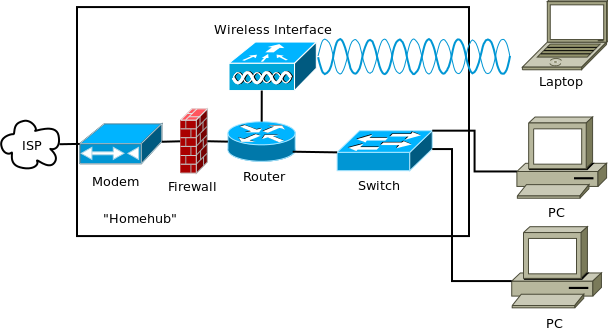
\includegraphics[width=\linewidth]{../Diagrams/Network/TypicalHomenet.png}
	\caption{The topology of a typical present day homenet.}\label{fig:typical_homenet}
\end{center}
\end{figure}

Modern home and small/home office (SOHO) \nomenclature{SOHO}{Small Office Home
Office} networks tend to follow a pattern. A single ISP provides internet
connectivity using the phone line or television cable.  The ISP typically
provides a single IPv4 address (/32).\footnote{This is CIDR notation, it
represents the number of bits used to identify the network the host.} Usually
this is an unstable (dynamic) allocation -- a static IP is usually only offered
as a premium service. 

To allow multiple hosts on the network, Network Address Translation (NAT)
\nomenclature{NAT}{Network Address Translation} is usually employed. With NAT,
the router rewrites the address of the packets from the global IP address to a
local IP address. The private address range 192.168.1.0/24 is often used for
local IP addresses. Ports number are regularly used to multiplex between the
different hosts and applications on the network. To allow programs like Skype
to function, Universal Plug and Play (UPnP) \nomenclature{UPnP}{Universal Plug
and Play}, a technology that allow automatic port mapping on a network, is
frequently deployed. Local IP addresses are assigned to the hosts by the router
using the Dynamic Host Configuration Protocol (DHCP)\nomenclature{DHCP}{Dynamic
Host Configuration Protocol}. 

A single item of Customer Premises Equipment (CPE) \nomenclature{CPE}{Customer
Premises Equipment} is usually supplied to the customer. These devices are
referred to by many names,\footnote{Names include Super Hub, HomeHub and
WirelessBox} but most commonly as a ``Router''.  This device provides the modem for
connecting to the internet, an Ethernet switch with around four ports, and a
wireless access point (802.11) that tends to be bridged to the wired network to
provide just one subnet. A typical home network topology is shown in
Figure~\ref{fig:typical_homenet}.

\section{Campus and Enterprise Networks}
\begin{figure}
\begin{center}
	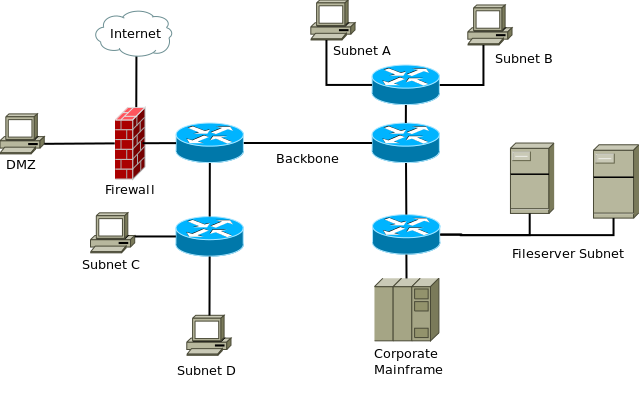
\includegraphics[width=\linewidth]{../Diagrams/Network/CorporateNetwork.png}
	\caption{The topology of a typical corporate network.}\label{fig:corporate_net}
\end{center}
\end{figure}
Larger networks like the ones found on university campuses and larger
businesses employ many of the more advanced features of networking.  Multiple
subnets separate hosts based on their physical locations, work groups and
expected uses. One potential corporate network topology is shown in
Figure~\ref{fig:corporate_net}.

In the early days of the internet, many organisations were issued large chunks
of IPv4 address space -- MIT famously has the control of a /8 address
range\cite{IPv4IANA}. The University of Southampton has a /16 (152.78.0.0),
providing around 65000 addresses. Having this many addresses allows each
machine on the network to be globally addressable -- a good firewall ensures
this is secure.  Even with this many addresses, the University still struggles.
This is due at part to address space wastage, the now deprecated ISS wireless
service still consumes a large proportion of the address space.

Running a network the size of the University's, based on today's technology
does require specialist staff to configure the network and ensure its
day-to-day operation. This is something that the vast majority of households do
not have.

\section{Future Networks}
\begin{figure}
\begin{center}
	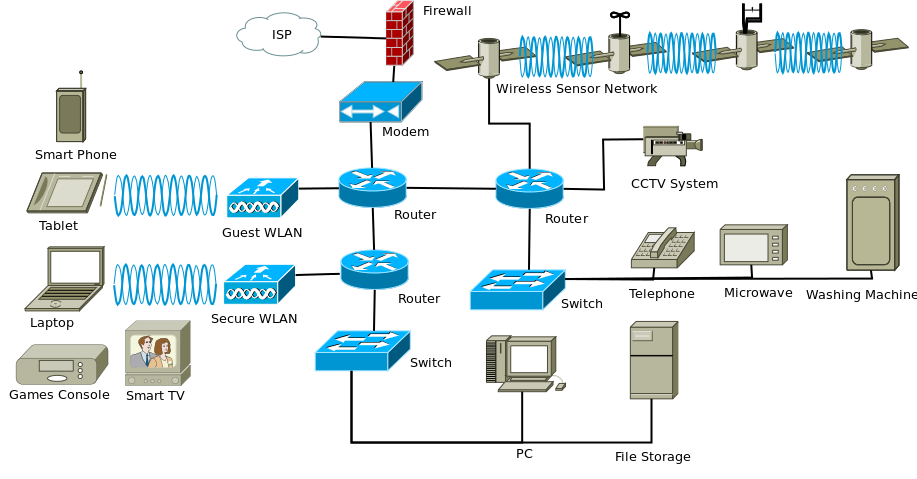
\includegraphics[width=\linewidth]{../Diagrams/Network/FutureHomenet.png}
	\caption{The topology of a hypothetical home network.}\label{fig:future_net}
\end{center}
\end{figure}
In the future users will expect more from their home networks. We are likely to
see dramatic increases in the number of devices in the average home, ranging
from more laptops, smart phones and tablets, to more sensors (e.g.\@
temperature/humidity) and home automation devices. Figure~\ref{fig:future_net}
shows a hypothetical future home network.

A home network with this quantity and heterogeneity of traffic is likely to
experience slow downs and other issues. These problems arise for two reasons:
Firstly sensor networks run very slowly, where as Gigabit Ethernet networks run
very quickly -- differences in speed can result in both networks running
slower. The other issue is the vast amounts of multicast and broadcast
traffic that will build up on networks with many devices performing functions
such as service discovery. It would be beneficial to split the network up into
multiple subnets to ensure the best performance from each network. 

Guest networks are already an option provided by some high end wireless access
points. By using Virtual Access Points (VAPs) \nomenclature{VAP}{Virtual Access
Point} guest clients can connect to the internet, but are restricted from
having access to the local network. To facilitate this, hard coded local
IPv4 addresses are usually used, with the advent of IPv6 and globally valid
addresses, a mechanism to assign IP addresses and route traffic is required. 

The Internet Engineering Task Force's (IETF) Homenet working group
\cite{homenet} are working on the architecture of the home network of the
future. Their work focuses on addressing, routing, topology and security
in home networks. 

\section{IPv6}
To communicate with a computer, a way of uniquely identifying it is required.
Currently, IPv4 is the dominant technology for addressing computers. When IPv4
was designed, it was not foreseeable that we 4 billion addresses would be
needed, so a neat 32 bit identifier was used.  In 2011 the Internet Assigned
Numbers Authority (IANA) \nomenclature{IANA}{Internet Assigned Numbers
Authority} ran out of IPv4 addresses \cite{potaroo}. 

One solution to the IPv4 address space exhaustion problem is migration to IPv6.
IPv6 is fundamentally similar to IPV4, but uses larger 128 bit addresses. This
gives us far more addresses to work with -- a total of $3.4028237\times10^{38}$
unique addresses. With estimates for the total number of grains of sand on
Earth being around $7.5\times10^{18}$, the number of stars visible from Earth
falling at about $7.0\times10^{22}$, and the estimated population of Earth
being a mere $7.0\times10^{9}$, this address space should be sufficient for at
least the foreseeable future. 

IPv6 address ranges are given in Classless Inter-Domain Routing (CIDR)
\nomenclature{CIDR}{Classless Inter-Domain Routing} notation. In this notation
an IPv6 address is followed by a slash and a number between 0 and 128 that
represents the number of bits in the IPv6 address that identify the network --
the remaining bits identify the host. CIDR notation replaces subnet masks used
in IPv4.

IPv6 prefixes tend to be /64, as this is required by Stateless Address
Autoconfiguration (SLAAC)\nomenclature{SLAAC}{Stateless Address
Autoconfiguration}. A /48 prefix may be allocated by an ISP to allow the user
to assign multiple subnets on their network.

The networks run by ECS are dual stack: the machines have both IPv4 and IPv6
addresses. Although this is not yet common place, 6\textsuperscript{th} June
2012 was World IPv6 Launch; many websites, including Facebook and Google, began
offering IPv6 connectivity\cite{IPv6Launch}. This demonstrates that IPv6 is
mature enough to be deployed in large networks.

\section{Routing}
For packets of data to find their way between subnets, they require routing.
We are concerned with Layer 3 (Network/IP Layer) routing.\footnote{For a brief
explanation of OSI layers see Appendix~\ref{osi}} When an IP packet is sent
(or forwarded), its address is compared with those stored in the kernel's
routing table, and then transmitted using the appropriate interface. Networks
contain many computers, known as routers, whose sole purpose is to forward
network traffic.

Several protocols exist to build up these routing tables:

\subsection{Interior gateway protocols}
Interior Gateway Protocols (IGPs) \nomenclature{IGP}{Interior Gateway
Protocols} build routing tables for a single autonomous system (AS)
\nomenclature{AS}{Autonomous System}. ASs are generally managed by ISPs or
other very large organisations.  

\subsubsection{Distance Vector}
Distance vector routing works by having each router advertise to its neighbors
(directly connected routers) the shortest path it knows about to each subnet.
Although less complex than link-state routing protocols, they are often slower
to converge, and experience the ``count to infinity'' problem whereby loops in
the network topology can lead to weights increasing to infinity when a router
goes down. 

The most common distance vector protocol is Routing Information Protocol
(RIP).\nomenclature{RIP}{Routing Information Protocol}\footnote{The routing
protocol famous for defining 15 as infinity.} The latest revision is RIP Next
Generation (RIPng) which offers IPv6 support. IGRP and EIGRP are Cisco's own
proprietary alternatives.

\subsubsection{Link-State}
In a link state routing protocols each router on the network builds a full
``map'' of the network topology. From this representation of the network, the
router calculates the best routes. The two most common Link-State routing
protocols, Open Shortest Path First (OSPF) \nomenclature{OSPF}{Open Shortest
Path First} and Intermediate System to Intermediate System (IS-IS),
\nomenclature{IS-IS}{Intermediate System - Intermediate System} both use
Dijkstra's algorithm to calculate these shortest paths. 

OSPF and IS-IS are very similar protocols, the main difference is that IS-IS as
a Layer 2 protocol is Layer 3 agnostic, whereas OSPF is dependent on IPv4 or
IPv6 depending on the version.

\subsection{Exterior Gateway Protocols}
Exterior Gateway Protocols (EGP) \nomenclature{EGP}{Exterior Gateway Protocol}
are used to establish peerings between ASs. EGPs typically run only on edge
routers and construct the route tables based on policy rather than the
technical distance of the destinations. In this project I was not concerned
with this kind of routing protocol.  The most widely used EGP is Border
Gateway Protocol (BGP)\nomenclature{BGP}{Border Gateway Protocol}.



\chapter{Literature Review} 
The project was based on two closely related internet drafts, they were both
published very recently, and share authors. If these drafts are approved by the
IETF they will become Request for Comments (RFC)\nomenclature{RFC}{Request for
Comments}, the technical documents that specify how the internet works. As RFCs
these documents will be placed on the standards track and will be labeled as
``Proposed Standards''. If they are successful in meeting certain criteria,
they may eventually become ``Internet Standards''\cite{rfc6410}.

\section{OSPFv3 Autoconfiguration}
Lindem and Arkko\cite{draft-ietf-ospf-ospfv3-autoconfig-02} describe how OSPFv3
can be extended to run without requiring configuration. The draft begins
by enforcing some default values, and restricting a few features -- such as
allowing only the backbone area to be used. It then specifies a mechanism for
generating Router IDs (RID) \nomenclature{RID}{Router ID} and ensuring that
there are no conflicts across the network. This is achieved by the introduction
of a new Link State Advertisement (LSA) \nomenclature{LSA}{Link State
Advertisement} type -- the Autoconfiguration LSA. 

The most recent release of this document was on 15\textsuperscript{th} April
2013. Although this was towards the end of my project, the changes were only
minor and I was able to incorporate them into my implementation.

\section{OSPFv3 Prefix Assignment}
Building on the work of the Autoconfig draft, Arkko, et
al.\cite{draft-arkko-homenet-prefix-assignment-03} solve the issue of
delegating IPv6 network prefixes from a larger pool of IPv6 addresses. As well
as offering a realistic solution to a problem, the draft also demonstrates the
extensibility of the Autoconfig draft. 

A method for breaking up a short prefix delegation into many network prefixes
is given, along with a strategy for avoiding conflicts across the network.
Typically an ISP will allocate customers a /48 IPv6 prefix to cover their
whole home, each network in their home then requires a /64 IPv6 prefix.

An update to this document was published on 23rd October 2013, it expired on
26\textsuperscript{th} April 2013, although it is likely a refresh will be
released soon.

\section{Other Important Drafts}
There are several other documents that are relevant to this project. These are
articles that are relevant as background knowledge and papers that have
been referenced from one another.

\subsection{Home Networking Architecture for IPv6} 
Chown, et al.\cite{draft-ietf-homenet-arch-07} put forward a vision of future
home networking. An architecture for future home networks is proposed, along
with a discussion of emerging technologies. 

\subsection{OSPF Version 2}
I studied RFC2328\cite{rfc2328} in depth to understand the OSPF Protocol. The
memo is surprisingly easy to read, and offers a complete discussion of the data
structures and algorithms the OSPF protocol employs to build routing tables for
IPv4. 

Although the document contains many details that are irrelevant to this project, 
including a long discussion on areas, and details of the SPF algorithms, I found
the understanding I gained through studying it invaluable to my project.

\subsection{OSPF for IPv6}
RFC5340 defines OSPFv3\cite{rfc5340}; it builds on RFC2328, to give the
reader a clear understanding of OSPFv3 by explaining the differences between
from OSPFv2. 

\subsection{Zeroconfiguration OSPF}
Dimitrelis\cite{draft-dimitri-zospf-00} published a draft in 2002 with similar
aims to the OSPFv3 Autoconfig draft, but focused on automatic configuration of
both IPv4 and IPv6, making it a more complex and restrictive solution. 

\subsection{The OSPF Opaque LSA Option}
RFC5250\cite{rfc5250} introduces the opaque LSA\@. An opaque LSA is a generic
LSA type that can be used to transmit application specific data. The concept is
similar to that used in the autoconfig draft, but it does not make use
of Type-Length-Values (TLVs)\nomenclature{TLV}{Type-Length-Value}. I found the
discussion about the reachability of LSAs useful.

\subsection{Additional Reading}
While learning about this area of networking, there were many other documents
that were either referenced from the more relevant drafts or defined a concept
that had been mentioned. This list includes:

\begin{itemize} 
  \item {\bf RFC 5838} Support of Address Families in OSPFv3 \cite{rfc5838}
	\\ Extensions to allow different kinds of address in OSPFv3.
  
\item {\bf RFC 6506} Supporting Authentication Trailer for OSPFv3  \cite{rfc6506}
	\\ Adds security back into OSPFv3.

	\item {\bf RFC 3630}  Traffic Engineering Extensions
	for OSPF \cite{rfc3630} 
	\\ (Updated by 4230 \& 5786) \cite{rfc4230}\cite{rfc5786} 
	\\ Adds LSAs to pass information for traffic shaping etc.\@
  
\item {\bf RFC 4862} IPv6 Stateless Address Autoconfiguration (SLAAC) \cite{rfc4862}
	\\ Explains how IPv6 networks can be established using NDP.\@

\end{itemize}

\section{Books}
There were a few books that were relevant to this project:
\begin{itemize}
  \item OSPF: Anatomy of an Internet Routing Protocol \cite{OSPFAIRP}
  \item OSPF: Complete Implementation \cite{OSPFCI}
  \item OSPF and IS-IS \cite{OSPFvsISIS}
\end{itemize}

These books were useful for clarifying things that were not clear from the
RFCs. They were also useful for reinforcing my general understanding of the
protocol, as they gave good overviews, written from different angles. 

Unfortunately the books did not cover OSPFv3 extensively because it is a
relatively recent development. There was no mention at all of more recent
drafts since they are very much on the cutting edge.

\chapter{Analysis}
\section{Alternatives}
There are other approaches that can be used to solve the problems addressed by
these drafts. The different solutions all have their merits -- to get a full
understanding of the problems with each approach, implementation is necessary.

\subsection{IPv4 Address as Router ID}
One possible solution to the RID assignment problem would be simply to use the
local IPv4 Address of the routers first interface. IPv4 Addresses seem like a
good candidate for the RID as they are both locally unique 32 bit identifiers.
This solution would be likely to provide a unique ID that does not require
configuring by the user.
 
However, as we enter a world dominated by IPv6, the use of IPv4 addresses will
diminish. IPv6 addresses are a poor candidate for RIDs for many reasons.
Firstly as they are larger than 32 bits, it would be difficult to create an
identifier certain to be unique from them. Secondly an interface is likely to
have many IPv6 Addresses. Of these addresses the only address it is guaranteed
to have is a link-local address, which does not have to be unique across the
network. 

\subsection{DHCPv6-PD}
\begin{figure}
\begin{center}
	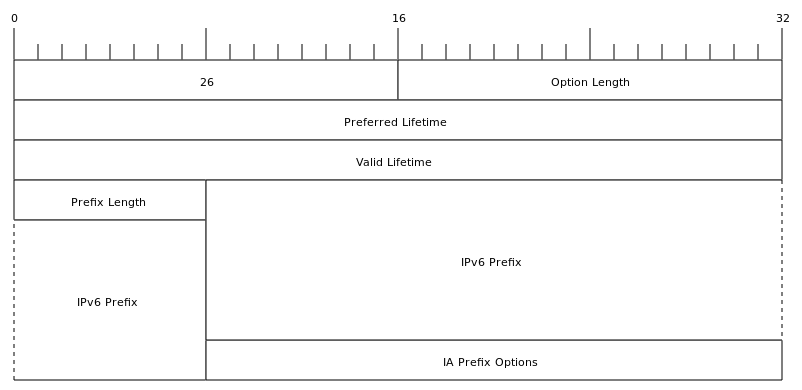
\includegraphics[width=\linewidth]{../Diagrams/Packets/pd-option.png}
	\caption{The DHCPv6-PD option.}\label{fig:pd-option}
\end{center}
\end{figure}
DHCP for IPv6 Prefix Delegation (DHCvP6-PD)\nomenclature{DHCPv6-PD}{DHCP for
IPv6 Prefix Delegation}, is a method for handing a prefix from one router to
another. The receiving router decides how it wishes to hand out the prefixes
contained in the prefix of the PD message (Shown in Figure~\ref{fig:pd-option}). 

One solution to the prefix assignment issue is using a hierarchical system.
Each router splits the prefix received from an upstream router and delegates an
equal size prefix to each downstream router. A positive side of this approach
is that it is very simple. The negative is that if the network is unbalanced,
one side of the network would be delegated a far larger address space than it
requires, while the other side is starved of prefixes.  Without some extension
there is no way of communicating address space requirements to upstream
routers.   

\subsection{Manual Configuration}
Another option is to accept that as networks become more complex, they will
require more configuration. In current home networks, most end users do not
understand how their network works, and have no desire to touch the
configuration anyway. Home users may end up with a better experience if a
trained engineer was sent by their ISP to set up their home network for them.
This would lead to more jobs, but would be inconvenient and expensive for end
users.

\subsection{Other Routing Protocols}
Other routing protocols make good candidates for this kind of solution. OSPF
was chosen as it as an IETF standard with good convergence rates and does not
suffer from many problems due to misconfiguration of the network -- such as
plugging multiple interfaces into the same link. Regardless of the routing
protocol chosen as the eventual standard in home networks, this project will
help influence its design.

\section{How OSPF works}
Open Shortest Path First (OSPF) is a link-state routing protocol. An image of
the whole network is built up by flooding Link State Advertisements (LSA)
across the network. Dijkstra's algorithm is used to generate routing tables from
the LSAs.

Several different message types exist in OSPF\@. These include:
\begin{itemize}
 \item Hello -- Sent out periodically to discover new adjacencies.
 \item Database Descriptions -- Which lists the LSAs in the routers LSDB (see below).
 \item Link State Requests -- Used to ask a router to send an LSA.
 \item Link State Updates -- Used to send an LSA.
 \item Link State Acknowledgments -- Sent on the receipt of an LSU.
\end{itemize}

The routers store known LSAs in their Link State Database
(LSDB)\nomenclature{LSDB}{Link State Database}. To identify which router
originated an LSA, each router is given a unique RID.

\subsection{Links State Advertisements}
\begin{figure}
\begin{center}
	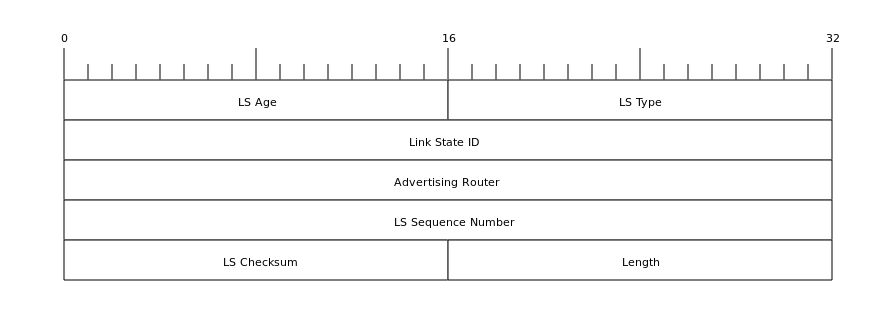
\includegraphics[width=\linewidth]{../Diagrams/Packets/LSA-header.png}
	\caption{OSPFv3's LSA Header.}\label{fig:LSA-header}
\end{center}
\end{figure}
There are many different LSA types in OSPF\@. Each LSA is originated by
a router on the network and forwarded by others depending on its
flooding scope. Each LSA contains some information about the network. 
 
The two most important LSA types are the Router LSA and the Network LSA\@.
Together they can be used to build up a complete picture of the
areas\footnote{Areas are an advanced OSPF feature used to reduce routing
protocol noise on very large networks.} the router belongs to.
Figure~\ref{fig:LSA-header} shows the structure of an LSA header. 

\subsubsection{Router LSA}
The Router LSA is originated by each router and is flooded across its own area.
Router LSAs contain information about the state of the router and its
capabilities. They also contain information about the interfaces attached to
the router, their types, and associated metrics.

\subsubsection{Network LSA}
Network LSAs are originated for each subnet, they are flooded to its own
area.  The only router that should originate this LSA is the Designated Router
(DR) \nomenclature{DR}{Designated Router}, and is elected with the DR Election
algorithm. The Backup Designated Router (BDR) \nomenclature{BDR}{Backup
Designated Router} is elected in a similar way, and must be prepared to start
emitting a Network LSA if the DR becomes unreachable. 

The Network LSA contains a list of routers connected to the subnet. There are no
weights associated with these connections as they are covered by the Router
LSAs. 

\subsubsection{Other LSAs}
Several other LSA types exist, many of them irrelevant to this project as they
are concerned with networks that consist of many areas, or interactions that
occur outside of the current Autonomous System (AS). Since OSPFv3 Autoconfig
dictates that only one area shall be used, these LSA types can be ignored.   

\subsection{Differences between OSPFv2 and OSPFv3}
The main difference is that OSPFv2 is for IPv4 and OSPFv3 is for IPv6. Some
more subtle changes include:

\begin{itemize}
	\item Additional and altered LSA types.
	\item Flooding scope now indicated by explicit option bits.
	\item Use of link local addressing.
\end{itemize}

\section{Implementation Candidates}
Below is a list of Open source implementations of OSPFv3\@. There are also
commercial implementations,\footnote{Most notably the one provided with Cisco
routers.} these have not been considered as they are closed source. 

\subsection{Bird}
Bird\cite{BirdHome} is a lightweight suite of routing protocols, written
in C. 

Bird has two implementations of Autoconfiguration OSPFv3. The first was written
in C as a separate branch. The other, extended Bird to allow LSAs to be
processed by external programs, and then used Lua to implement the drafts.

\subsection{Quagga}
Quagga\cite{QuaggaHome} is a more heavyweight package, it is a fork of now
defunct GNU project Zebra. Quagga is written in C, and aims to be
compatible with many platforms so does not rely on many external libraries.
Quagga has no public implementations of autoconfig OSPFv3.

\subsection{XORP}
XORP\cite{XORPHome} is another heavy implementation. It is written in C++,
there are no public Autconfig OSPFv3 implementations based on XORP\@. The
activity surrounding XORP is low. 

\section{Chosen Implementation}
I chose to base my project on Quagga. After subscribing to all three developer
mailing lists, Quagga seemed to be the most active project.  I also liked the
clear separation between OSPFv2 and OSPFv3 that Quagga offered.  Finally Quagga
is a good choice as there were no existing implementations of autoconfig OSPFv3
based on Quagga, so my contributions would be more useful to the community.

\chapter{Specification}
To direct the implementation and allow a thorough evaluation, I produced the
following specification based on the referenced drafts. To limit
ambiguity in requirements levels, I have used the language recommended by BCP14.
\cite{rfc2119}

My implementation:
\begin{enumerate}
	\item \textbf{MUST} allow the routing daemon to run without manual configuration.
	\item \textbf{MUST} resolve RID conflicts if they occur.
	\item \textbf{MUST} efficiently distribute IPv6 Prefixes across the network.
	\item \textbf{MUST} store assigned prefixes in non volatile storage.
	\item \textbf{SHOULD} be interoperable with existing implementations of the drafts.
	\item \textbf{SHOULD} generate a ULA if one is required.
	\item \textbf{MAY} emit RAs for assigned prefixes.
	\item \textbf{MAY} support source based routing.
	\item \textbf{MAY} obtain aggregated prefixes through DHCP-PD. 
	\item \textbf{SHOULD} be well tested, to ensure valid operation.
\end{enumerate}

\chapter{Design}
\section{Simplifications}
To allow OSPFv3 to function without configuration, a number of simplifications
must be made to how it runs. These simplifications restrict some of the fine
tuning required by large enterprise networks, but should not remove functions
exploited by home users. 

\subsection{Operation on One Area}
As the networks that are being configured are unlikely to be very large, there
is no benefit gained by using areas. In Autoconfig OSPFv3, all
interfaces on all routers will be part of Area 0.0.0.0, the backbone area.

Removing multiple areas also reduces the complexity in other aspects. Various
summary LSA types are no longer needed, and the area flooding scope now covers
the whole network.

\subsection{Default Values}
The draft specifies the use of default values. These are mainly values that were
optional in the original RFCs, and are now obligatory defaults for Autoconfig
OSPFv3\@. 

Firstly, with the exception of those that clearly should not run OSPF, (e.g.\@
manually configured, or connected directly to an ISP), all interfaces
should be automatically configured as the correct type. Most implementations
already do this. 

Secondly, defaults \texttt{HelloInterval} of 10 seconds, and
\texttt{RouterDeadInterval} of 40 seconds should be used. There is also an
optional reduction of the router inactivity timer from
\texttt{RouterDeadInterval} down to a minimum of \texttt{HelloInterval} + 1
seconds. 

Finally, with regard to OSPFv3 Address Families, all interfaces should use the
default value of 0 as their Interface Instance ID\@, to indicate that the
interface uses unicast IPv6.  

\section{New LSA Type}
\begin{figure}
\begin{center}
	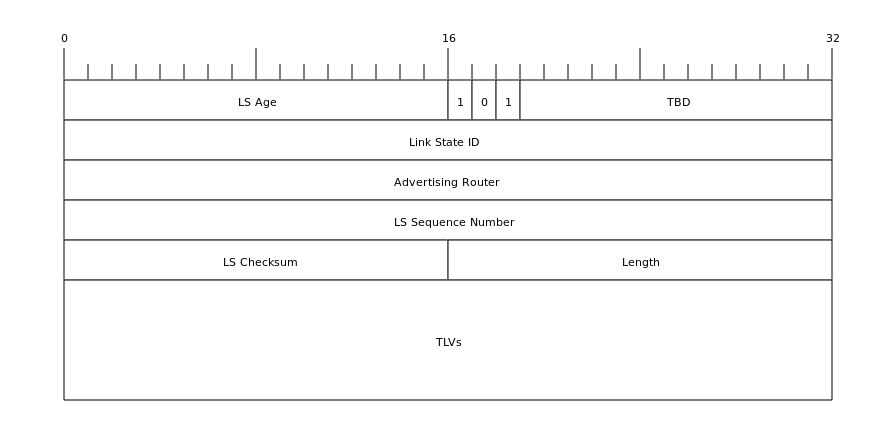
\includegraphics[width=\linewidth]{../Diagrams/Packets/ac_lsa.png}
	\caption{The new AC-LSA added by the Autoconf draft.}\label{fig:AC-LSA}
\end{center}
\end{figure}

The OSPFv3 Autoconfig draft specifies a new LSA type to ensure that
there are no conflicts in RID across the network. This new LSA is known
as an Auto Configuration LSA and currently uses an experimental Type value. A
value will be assigned by IANA when the draft is upgraded to an RFC. 

The AC-LSA is designed to be extensible, allowing for more uses to be added in
the future. The structure of an AC-LSA can be seen in Figure~\ref{fig:AC-LSA} 

\subsection{TLVs}
\begin{figure}
\begin{center}
	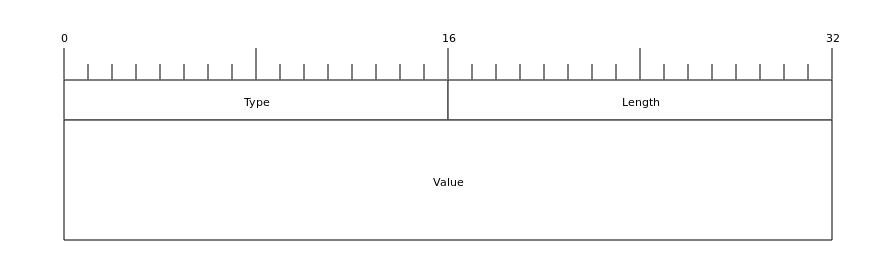
\includegraphics[width=\linewidth]{../Diagrams/Packets/tlv.png}
	\caption{The Structure of a TLV contained in an AC-LSA\@. Value has a variable
	size and is padded to the nearest 32 bits.}\label{fig:TLV}
\end{center}
\end{figure}

The payload of the AC-LSA is a set of Type-Length-Values (TLV). Each TLV
contains: 
\begin{itemize}
    \item The type of the data.
    \item The length of the value in bytes.
    \item The data itself.
  \end{itemize}

A diagram of the TLV's structure can be been in Figure~\ref{fig:TLV}

\subsubsection{Router-Hardware-Fingerprint TLV}
\begin{figure}
\begin{center}
	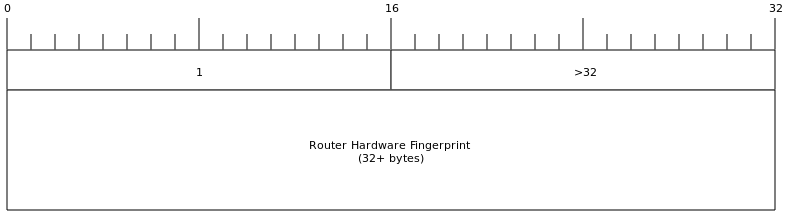
\includegraphics[width=\linewidth]{../Diagrams/Packets/rhwfp_tlv.png}
	\caption{A router-hardware-fingerprint TLV.}\label{fig:RHWFP-TLV}
\end{center}
\end{figure}
The Router-Hardware-Fingerprint (RHWFP) TLV (Figure~\ref{fig:RHWFP-TLV}),
specified in the Autoconfig draft, contains a unique identifier for its
originating router that is valid across the whole network. The RHWFP TLV is
used to ensure that the network is free from RID conflicts.

\subsubsection{Aggregated Prefix TLV}
\begin{figure}
\begin{center}
	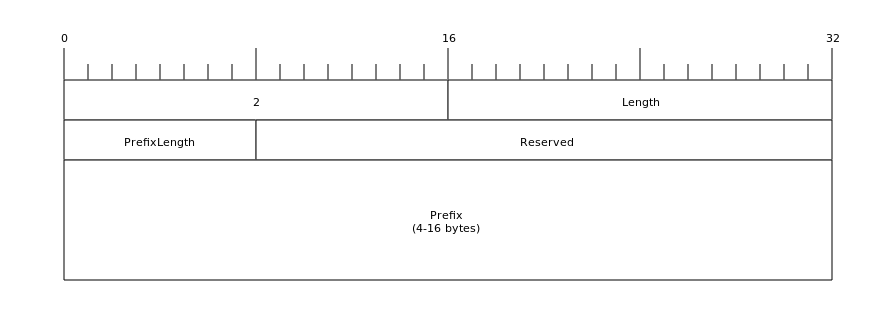
\includegraphics[width=\linewidth]{../Diagrams/Packets/aggregated_prefix_tlv.png}
	\caption{An aggregated prefix TLV.}\label{fig:AggregatedPrefix-TLV}
\end{center}
\end{figure}
The Aggregated Prefix TLV (Figure~\ref{fig:AggregatedPrefix-TLV}) is defined in
the Prefix Assignment draft, it represents a short IPv6 prefix delegation that
can be used to assign prefixes to the different subnets. 

An aggregated prefix should have a length of less than or equal to /64.
Typically an ISP will provide a /48. Aggregated prefixes have many possible
sources, the main two are DHCPv6-PD and manual configuration. 

\subsubsection{Assigned Prefix TLV}
\begin{figure}
\begin{center}
	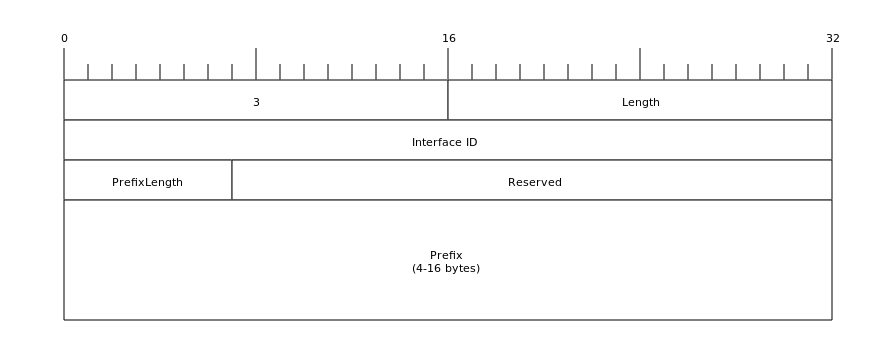
\includegraphics[width=\linewidth]{../Diagrams/Packets/assigned_prefix_tlv.png}
	\caption{An assigned prefix TLV.}\label{fig:AssignedPrefix-TLV}
\end{center}
\end{figure}
The Assigned Prefix TLV (Figure~\ref{fig:AssignedPrefix-TLV}) is also defined
in the Prefix Assignment draft. A router adds an Assigned Prefix TLV to its
AC-LSA when it makes an assignment from an Aggregated prefix. Each assignment
is made to one interface, and is a /64 as this is the length used by SLAAC\@.
Conflicts are resolved automatically if they occur. 

\chapter{Implementation}
Over the course of the project I produced and tested an augmented version of
the Quagga routing daemon. My changes consisted of adding $\mysym1,900$ lines
of C code to the \texttt{ospf6d} code base along with $\mysym400$ lines to
\texttt{zebra} and \texttt{lib}. I also modified existing code. $\mysym600$
lines of code were used for unit testing.

\section{Core Algorithms}
Several algorithms are used in Autoconfig OSPFv3 to ensure that the network
is configured correctly.

\subsection{Router-Hardware-Fingerprint Generation}
The Router-Hardware-Fingerprint (RHWFP) is a value that is based on properties of
the router that has a high probability of being unique across the network. 

I chose to use a concatenation of hashes of the MAC \nomenclature{MAC
Address}{Media Access Control Address} addresses of the attached interfaces.
MAC addresses are not totally guaranteed to be unique as manufacturers could
cut corners, but if they are not, we face much bigger problems in lower layers.

\subsection{Router ID Generation}
Autoconfig OSPFv3 says the RID should be a pseudo-random number, based on
the RHWFP\@. As the router will need to reassign its RID a new value if
there is a conflict, a seed value must be stored. This value is passed by
reference to the \texttt{rand\_r} function call, which modifies it to maintain
the state of the random sequence.

One difficult part of the project was cleanly shutting down OSPFv3, changing
the RID, and then bringing it back up. 

\subsection{Router ID Conflict Resolution}
As the RIDs are random, there is a possibility of a collision -- two
routers on the network assigning themselves the same RID\@. To prevent
things going awry a mechanism for resolving these conflicts is needed. 

The draft specifies two mechanisms for detecting and resolving conflicts. 

\subsubsection{Local Collisions}
A local collision, where there is an adjacency\footnote{Routers are
directly connected.} between the conflicting routers, is detected when any
valid LSA is detected to have the same RID but a different Link-Local
IPv6 address. To resolve this conflict, the router with the numerically lower
Link-Local Address generates a new RID\@. 

\subsubsection{Network-Wide Collisions}
To detect collisions that occur for routers that are not directly connected,
all apparently self originated AC-LSAs are inspected to ensure that the RHWFP
match. If they do not then the router with the lower RHWFP must change its
RID.

\subsection{Prefix Assignment}
When a router notices a change in the current set of AC-LSAs in the LSDB, the
prefix assignment algorithm is scheduled to run. Scheduling uses Quagga's built
in thread library and has the benefits of allowing the code to finish whatever
it was doing and ensures the algorithm is only run once if it is scheduled many
times in close succession.

The algorithm examines all aggregated prefix interface pairs. If there is not
already an assignment for the pair, and the router has the highest RID of all
active neighbours on that link, then a prefix is assigned to the interface from
the aggregated prefix. 

There is no prescribed method in the draft for making an assignment, beyond
that the prefix assigned must not be in use. I wrote my implementation to
ensure it is easy to change the method used for picking a new prefix for the
assignment. 

I chose to step through the prefixes in numerical order. The disadvantage is a
high likelihood of collision with a router elsewhere in the network; this was
advantageous during the testing phase as it makes these cases more common,
leading to easier testing. The other advantage is that this algorithm is
guaranteed to either find a free address, or produce an error if the address
space has been exhausted. 

\subsection{Prefix Conflict Resolution}
Prefix collisions occur either when multiple routers have used the same prefix for
different networks, or multiple routers have assigned different prefixes to the
same network. The prefix assignment algorithm is designed so that these
collisions are resolved during assignment. Routers will only accept the prefix
assignment made by the router with the highest RID of the assigning routers. If
a router detects that one of its own assignments is no longer valid, it will
deprecate it and reschedule the algorithm. 

\subsection{Making an Assignment}
\label{pending_list}
The prefix assignment draft specified a hysteresis period of 20 seconds
before an assignment is committed to. The draft does not explain exactly what
is meant by this. My implementation uses a list to indicate that a prefix is
pending, so that if it needs to be deleted it can be deleted immediately. After
20 seconds is up, the prefix is removed from the pending list and Router
Advertisements (RA) are emitted containing the prefix.
 
\subsection{Deprecating an Assignment}
When the prefix assignment is run, all existing prefix assignments are first
marked invalid. As the algorithm runs, the prefixes that are found to be valid
are marked as such. If by the end of the algorithm a prefix is still marked
invalid, deprecation is scheduled. 

If after 240 seconds has passed, the prefix is still marked invalid, it is
deleted from the interfaces list of assigned prefixes and an RA is broadcast
with the lifetime set to zero. 

\subsection{ULA Prefix Generation}
If a there are no aggregated prefixes in the routing domain after 20 seconds,
the router with the highest RID must generate a Unique Local Address
(ULA)\nomenclature{ULA}{Unique Local Address} prefix\footnote{In the defining
RFC these are referred to as Global IDs.} to facilitate local connectivity.
ULAs are similar in concept to IPv4 Private addresses (e.g.
192.168.1.0).\footnote{Although it is not recommended to use NAT with IPv6}

The ULA prefix generation algorithm is defined in RFC4193 (Section
3.2)\cite{rfc4193}. It attempts to generate a unique /48 prefix, based on a
hash of a portion of a combination of the current network time (in Network Time
Protocol (NTP) \nomenclature{NTP}{Network Time Protocol} format), and an
interface's 64-bit MAC address (EUI-64).\nomenclature{EUI-64}{Extended Unique
Identifier}

Once a ULA prefix has been generated it is advertised as an aggregated prefix.
If a router with a higher RID becomes reachable, or an aggregated prefix is
received from another source, the prefix is deprecated after 120 seconds. The
draft recommends that ULAs are deprecated if there are any global addresses in
the system,to prevent local IPv6 islands forming -- this is an area of debate
within the IPv6 community. 

\subsection{Source Based Routing}
\label{SourceBasedRouting}
\begin{figure}
\begin{center}
	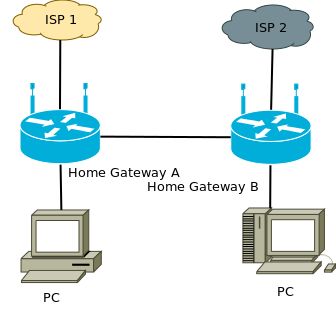
\includegraphics[width=\linewidth]{../Diagrams/Network/MultipleISP.png}
	\caption{An example of a home network with mutliple ISPs.}\label{fig:MultipleISP}
\end{center}
\end{figure}
In the future it may become common for households to have multiple internet
connections, as shown in Figure~\ref{fig:MultipleISP}. For example, a cable
connection with ADSL for backup could provide households with a resilient
connection. 

To prevent various attacks,\footnote{Denial of Service
(DoS)\nomenclature{DoS}{Denial of Service} attacks using spoofed source
addresses are common.} in accordance with BCP 38\cite{bcp38}, ISPs will not
forward traffic with a source address outside the prefix allocated to that
network. As such, if multiple ISPs are used, network traffic must be routed to
the correct ISP\@. Source based routing aims to solve this problem by considering
the source address, as well as the destination. 

I implemented a proof-of-concept based on my autoconfig code. This branch is
incompatible with my unaltered autoconfig implementation. It is based loosely
on work by Baker \cite{draft-baker-ipv6-ospf-extensible-00}
\cite{draft-baker-ipv6-ospf-dst-src-routing-00}, published
17\textsuperscript{th} February 2013, that specifies replacements for the
standard OSPFv3 LSA types, using Type Length Values (TLVs) similar to those in
the autoconfig draft. Due to the complexity of these drafts, I decided not to
conform to them in my proof-of-concept.

My implementation works by exploiting the Linux Kernel's ability to have
multiple routing tables. A routing table is created for each source address
range that will be routed. The system's policy table is then used to select
which routing table to use based on the source address.  

Quagga's Zebra daemon has the ability to manipulate any routing table. I
extended the Zebra protocol's message for adding entires to the routing table
to include the source address, and selected the routing table based on a hash
of this address. Unfortunately, Quagga cannot manipulate the policy table. To
overcome this I used \texttt{iproute2}'s \texttt{ip -6 rule} command, which I
called from a bash shell script, invoked using the \texttt{system} function. 

This proof-of-concept demonstrates that Quagga can be extended to implement
source based routing. It is not a complete solution -- firstly it is not
interoperable with other implementations as it does not conform to the draft.
Secondly using the \texttt{system} system call is not secure, elegant or
portable. 

\section{Quagga}
Quagga is written in C89, following the GNU coding
standards\cite{gnucodestandards}. These rules help to improve the portability
of the code, meaning that if there is a C compiler, and the operating system is
Unix-like, then Quagga is likely to compile for it.  Quagga does not
support Microsoft Windows.\footnote{Or WinDoze as the GNU coding standards would
put it}.

\subsection{Style}
At first I found some of the stylistic guidelines of the GNU coding standards
unusual and difficult to read, the following contributed to this:
\begin{itemize} 
  \item Space between function a call and its parameter list's opening parenthesis.
  \item Return type declaration on the line above the name of the function.  
  \item Opening curly brace of a block on a new line.
\end{itemize}

When I first opened one of Quagga's source files, it took me a short while to
realise that I was looking at a function declaration. Fortunately as time went
on, reading and writing this formatting became second nature to me. 

Being written in C89, Quagga is not object oriented. The structure of the code
however, does resemble object oriented programming. \texttt{struct}s are used
extensively to represent the ``objects'' in the program. Functions tend operate
on these \texttt{struct}s, in a similar way methods act on the objects
they belong to.

Working on a large and complex program was difficult, and determining the
correct level of abstraction for each function was tricky.  I felt I had to
work around the lack of inheritance and polymorphism to write clean code. 

When writing in a low level language like C, especially when the program will
have very long up times, ensuring that it is free from memory leaks is
important. If memory that is allocated using the \texttt{malloc} system call is
not deallocated using \texttt{free} then it will become unusable. This unusable
memory will build up, eventually the program will crash as the operating system
is unable to allocate it more memory.

\subsection{Quagga's Library}
Quagga tends to avoid relying on external libraries. There is a ``lib'' folder
in the source code repository that contains non-protocol specific code. This
library provides commonly used data structures and algorithms to the protocol
implementations. 

\subsubsection{Thread}
I made heavy use of the Thread library item. Threads are a similar to operating
system threads. They consist of pointers to functions that will be called upon
some event, or after a set time. These threads are an application level
construct. The program  executes as one process, so only one thing is being
executed at any given time. Although this means the multi-core architecture of
modern CPUs is not exploited, it simplifies development, removing the need to
worry about thread safety.

\subsubsection{LinkList}
Linklist was another useful element of the library. It implements a doubly
linked list -- a series of nodes with pointers to the next and previous node in
the list.  Variable length lists were required frequently in my program, and
Linklist worked well for this. Linklist also offers a macro
\texttt{ALL\_LIST\_ELEMENTS} that can be used like to Java's enhanced
\texttt{for} loop.\footnote{Variables to hold pointers to the current and next
node make it look messy though.} Linklist's main drawback is that due to
limitations of C, the data is referenced by a typeless pointer, and therefore
is not type safe. If the developer is careful this should not be an issue. 

\subsubsection{Prefix}
Another library component is Prefix. It represents an IPv4 or IPv6 address, and
offers several functions to perform on them. One of the most useful features is
the ability to convert between C strings (\texttt{char *}) and
\texttt{in6\_addrs} (the representation used in Unix-like kernels). This is
useful for user interface and debugging messages.  There are also
\texttt{memcmp} based macros available for testing whether two IP addresses are
the same. I extended Prefix to include a function that determined whether or
not a given Prefix contained another given Prefix.

\subsubsection{MD5}
The other interesting thing in the library is MD5
\nomenclature{MD5}{Message-Digest Algorithm 5}, which generates cryptographic
hashes. For the generation of ULAs, SHA-1 \nomenclature{SHA-1}{Secure Hash
Algorithm 1}, a similar but more secure hash, is recommended. As I did not have
a SHA-1 implementation, MD5 made an acceptable substitute. 

\subsection{vtysh}
\texttt{vtysh} \nomenclature{vtysh}{The Command Line Interface for Quagga} is a
Virtual Teletype shell. It is the primary interactive user interface for
Quagga. \texttt{vtysh} can be accessed locally on the router using the
\texttt{vtysh} command, or remotely using telnet. \texttt{telnet} connections
are made directly to the routing protocol daemon, i.e. \texttt{telnet ::
ospf6d}.  

The interface is based on Cisco's router's. Commands like ``\texttt{show ipv6
ospf6 database detail}'' can be used. ``\texttt{sh ipv os da de}''  
performs the same command as it is unambiguous. This command will
list out, in full detail, the contents of all of the LSAs that \texttt{ospf6d}
knows about. 

I added commands to \texttt{vtysh} that allow the user to list and add
prefixes. Details of this can be found in Appendix~\ref{vtysh}. 

\section{Router Advertisements}
Router Advertisements (RA) \nomenclature{RA}{Router Advertisement} are part of
the Neighbor Discovery Protocol (NDP), \nomenclature{NDP}{Neighbor Discovery
protocol} and are used to advertise network prefixes, and the address and
routing domains of the router making the advertisement. Upon receiving
an RA, a host should generate IPv6 addresses within the prefix being advertised. 

Typically routers use \texttt{radvd} \nomenclature{radvd}{The Router
Advertisement Daemon} to generate RAs. I felt coupling Quagga to another
piece of software would be undesirable. My reasons are firstly, that one cannot
be sure the package will always the most popular choice. Secondly, if the
API for \texttt{radvd} changes, then Quagga would also need to be changed. And
finally there do not seem to be any clean ways of interfacing with
\texttt{radvd}: the daemon must be halted, configuration files updated and then
started up again.

Fortunately Quagga has its own, slightly limited, code for emitting RAs. This
functionality is part of Zebra, the code responsible for updating the routing
table. The \emph{correct} way of accessing this functionality from within the
routing protocol implementation (i.e. \texttt{ospf6d}), is to send a message
using the library component \texttt{zClient}, which is then received and
enacted upon by \texttt{zServ}, part of Zebra. 

Initially the only way to set whether router advertisements were on or off, and
to set which prefixes the router advertised, was to use \texttt{vtysh}. I
extended the \texttt{zClient-zServ} protocol to include messages that expose
this functionality to the routing protocol implementations,
Appendix~\ref{zClient} contains details of these messages. 

\section{Endians}
An ongoing issue in my project was the storage of integers.  \ x86
architecture, found in modern desktop processors, is little endian.  This means
a value represented as multiple bytes, is stored with the least significant
(lowest in value) byte first. On the contrast when transmitting data using the
IP protocol, network byte order is defined as big endian -- the most
significant bytes are transmitted first. 

I had to be careful to convert to the correct endian; tiny mistakes lead
to a long time debugging. Fortunately for all the standard sized data types,
there are functions to convert the endian.  \texttt{htons} converts host shorts
(unsigned 16 bit integers) to network shorts; \texttt{ntohs} does the opposite.
\texttt{htonl} and \texttt{ntohl} work on longs (unsigned 32 bit integers). 

The benefit of having different endians on the network and the development
architecture is that ensures endians are considered. If the development platform
used the same endians as the network then it would be very easy to forget about
endians altogether. It would then cause serious problems when the software is
ported to a platform that uses different endians to the network.
    
\chapter{Testing}
To ensure that my code worked as I intended it to, it needed to be tested. 

\section{Assertions}
To ensure that my code failed early if something was wrong, I systematically
peppered my code with assertions. Assertions are statements that insist that
their predicate is true -- If the assertion is correct, execution continues as
normal, otherwise the program will halt.

Assertions in my code check for circumstances that should never occur. This
ensures that the code never executes in an invalid state, producing incorrect
results. 

\section{Unit Testing}
\begin{figure}
\begin{center}
	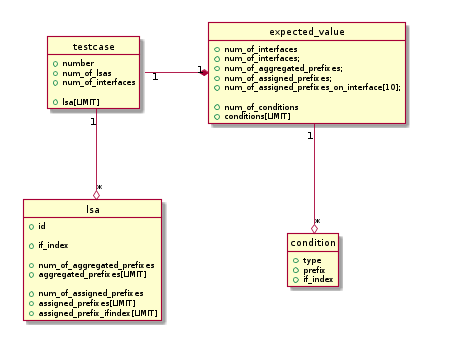
\includegraphics[width=\linewidth]{../Diagrams/Testing/testcase.png}
	\caption{A class diagram showing the structure of my unit testing code.}
	\label{fig:testcase}
\end{center}
\end{figure}
I created unit tests to ensure that my code behaved as expected, I focused
heavily on edge cases. Creating unit tests gave me confidence that my code did
what I intended it to do, however, it did not ensure that my intentions were
correct.

Although there are unit testing frameworks available for C, I decided against
using them.  I felt using external libraries  would go against the ethos of
Quagga, and my testing strategy did not fit the design of most popular
libraries. 

The design of my unit testing code is shown in Figure~\ref{fig:testcase}. A
summary of the results for my testing can be seen in
Appendix~\ref{testResults}.

\subsection{Test Cases}
Test cases are specified by \texttt{struct}s containing the parameters of the
system, this includes the number of interfaces and the set of LSAs in the
system. 

The test cases are used to construct a mock environment that resembles
Quagga during normal execution. This is done by populating the \texttt{struct}s
Quagga uses with fake data. The prefix assignment is run for each of the test
cases. 

\subsection{Expected Values}
Each test case has a corresponding expected value, consisting of a
series of system parameters and conditions. Once a test case has been run, if
the state of the mock environment is consistent with the expected value, the
test passes, otherwise it fails. 

\section{Netkit} 
\begin{figure}
\begin{center}
	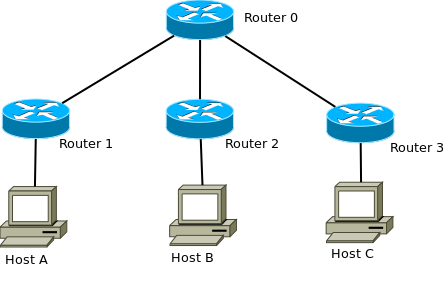
\includegraphics[width=\linewidth]{../Diagrams/Network/MainNetkit.png}
	\caption{The topology of the netkit network I used for most of my testing.}
	\label{fig:NetkitTopology}
\end{center}
\end{figure}
Netkit is a tool that allows developers to easily test network software and
configuration. Netkit uses User Mode Linux (UML) \nomenclature{UML}{User Mode
Linux} to run many Virtual Machines (VMs) \nomenclature{VM}{Virtual Machine}
on a single desktop PC. 

Netkit presents the user with an \texttt{xterm} window for each VM\@. These VMS
behave like normal Linux computers. They have virtual network interfaces, that
act much like real network interfaces. Netkit allows these virtual interfaces
to be joined together through collision domains -- setting two interfaces to
the same collision domain is like plugging two hosts into the same network
switch.  Netkit also provides a special type of collision domain called a
``tap''; this can be used to share the host computer's network connectivity
with the Netkit network.

Netkit provided me with an indispensable testing environment. I was able to run
an instance of Quagga on each virtual machine, and control them through
\texttt{vtysh}. Having seven terminal windows on a single computer is far more
convenient than having seven separate devices that must be configured
separately. Netkit's biggest advantage over using \texttt{ssh} or
\texttt{telnet} is that it does not  dependent on network connectivity, so you
are free to make changes to the network without losing your remote connection.

Compiling the code from within Netkit is also much faster than on the Alix2d3s
(See Section\ref{alix}), the difference was between several hours on the
Alix2d3s and several minutes in Netkit. This was because rather than using a
500MHz AMD Geode\footnote{A low power System-on-chip designed for the embedded
market in around 2002}, Netkit used my desktop PC's 3.3GHz Intel i5
2500k\footnote{A mid/high end desktop processor from 2011} for compiling. 

I found Netkit to be a great tool for understanding how networks work.
Translating my knowledge of network theory to an ability to configure real
networks was tough. Trivial things often turn out to be the issue -- an example
is setting \path{/proc/sys/net/ipv6/conf/all/forwarding} to 1, allowing IPv6
traffic to be forwarded. It is not an important piece of theory, but if it is
not done, routing will not work. 

\section{radvdump}
\texttt{radvdump} is a tool that shows the contents of all received router
advertisements. It is designed to be used with \texttt{radvd} and outputs the
contents of a RA in the style of a \texttt{radvd} configuration file, an
example is shows in Appendix~\ref{radvdump} 

I used \texttt{radvdump} to ensure that Quagga was successfully sending RAs and
the contents were as expected. 

\section{Tunnel Broker}
Using Hurricane Electric's (HE) Tunnel broker service, I was able to give my
network global connectivity. An HE tunnel, provides you with a single /64 IPv6
prefix. It is possible to request a larger /48 allocation. The tunnel is
configured at their end to route any traffic that is destined to your prefix,
to the endpoint that you specified.  

By configuring a static route forwarding all traffic for the allocated /48
prefix into the Netkit network, then setting up Quagga within the Netkit
network, using the allocated prefix as its aggregated prefix, I was able to
make the IPv6 addresses globally reachable. Using a remote server
(\texttt{uglogin}) I was able to ping the virtual devices, demonstrating that
the devices had global addressability.

\section{Alix2d3}
\label{alix}
Although I was confident that testing my code using Netkit was sufficient to
show it working correctly, I ran my code on two Alix2d3 devices. Alix2d3s are
very small computers on which one can install Linux. They make good routers as
they have multiple network interfaces. This offered more tangible proof
that my code functions correctly. It also allowed me to do things that home
users are likely to do, such as plugging the routers together in arbitrary
configurations.

Testing on the Alix2d3s was much more difficult and time consuming that testing
with Netkit, so I avoided doing the bulk of the testing this way. I employed a
black box testing approach, plugging the devices together and checking that
everything seemed to be working. 

\section{Interoperability}
One of the goals of my project was to verify that the implementations produced
by other developers were compatible with the code I produced. 

Both of the implementations I tested against were based on Bird. As Bird and
Quagga both implement the same specifications for OSPFv3, I felt it was safe to
assume that the unmodified versions Bird and Quagga would be compatible. 

\subsection{Ben's Implementation}
Ben Paterson's implementation\footnote{Available at:
\url{https://github.com/fingon/bird-homenet}} was written in C. I found it
easy to install onto my Netkit testbed -- I cloned the Git repository and
compiled the code in one of the Netkit VMs. 

Ben's implementation correctly implements the Autoconfig draft. However, I
discovered that my implementation was wrong: The RHWFP is defined as 32 bytes,
I had used as 32 bits. I modified my implementation to correct this, also
adding support for padded TLVs. After making the appropriate changes to my
implementation, the two worked well together for this draft.

Unfortunately, this implementation does not correctly implement the Prefix
Assignment draft. A fourth TLV type not present in the Prefix Assignment draft
is used. This TLV contains information about an interface, and is then followed
by a series of Assigned Prefix TLVs minus any interface information. 

Ben's implementation uses an interesting algorithm for assigning prefixes:
It begins by picking a prefix from the address range at random, it then checks
that this prefix has not already been used. If it conflicts then it picks
another at random. To ensure that this random process does not continue
indefinitely, after a certain number of attempts, the algorithm falls back to
picking the addresses sequentially. 

\subsection{Markus' Implementation}
Markus Stenberg's implementation takes an unusual approach to extending Bird. A
fork of Bird has been created called Bird-Ext-LSA\@,\footnote{Not to be
confused with External LSAs in OSPFv3 that carry information from other
protocols.}\footnote{Available at:
\url{https://github.com/fingon/bird-ext-lsa}} which offers a mechanism that
allows LSAs to be processed by a separate program. 

Bird-Ext-LSA is complimented by hnet-core\footnote{Available at:
\url{https://github.com/fingon/hnet-core}} (Homenet Core), which implements,
among other things, the Autoconfig drafts\@.  hnet-core is written in the
scripting language Lua. Running this code was a challenge -- I had problems
creating the right environment; the code has many dependencies,
\texttt{Luarocks} helped install some of these. 

Eventually I got the code running; without alteration, it was incompatible with
my implementation. To enable compatibility with a version created by the
draft's author (Jari Arrko), a different AC-LSA Type number was used -- this
confused me at first, but once spotted it was simple to fix.

The other compatibility issue was that this implementation interpreted the TLVs
length to include the TLV header. The draft explicitly states that the length is
of the value alone, so I corrected the code, to allow myself to continue
testing. The implementation relied on the interface ID being appended to the
TLV header rather than being part of the value, so the changes were harder than
they should have been.

After all this was fixed, there seemed to be a good level of compatibility,
with prefixes from one finding their way into the other.

\section{Further Testing}
To increase the confidence in my code to the level expected of a
commercial product, it would be wise to undergo further testing. 

One method of testing is to use a commercial network protocol compliance
verification suite, such as IxANVL or Spirent. These ensure that the protocol
conforms to the specification. This is currently not possible for my project as
the implemented protocol is not yet included in these suites.  Although there
is an open source library for testing OSPFv2, I was unable to find any open
source libraries for testing OSPFv3 that could be easily extended to test
autoconfiguration. 

Moving beyond this, some level of user testing should be undertaken before
publicly releasing this code, and integrating it into Quagga. Typically, code
undergoes closed Alpha testing by a small number of developers, followed by
Beta testing, where it is released to the public without guarantees of
correct functionality.

\chapter{Project Management}
\section{Tools}
A personal goal for my project was to use of lots of new tools. During the
project, I ended up using a wide variety of tools. Some of the tools I had used
before, but using them on a large project meant that I made use of features that
I did not know existed before.

\subsection{Git}
I chose to use Git as my version control system. This choice was
partially because Quagga uses Git, however there are many other good reasons for
using Git, or any other Distributed Version Control System (DVCS).
\nomenclature{DVCS}{Distributed Version Control System} 

Firstly, version control is essential to a software project as it enables the
developer to keep track of changes over time and revert to old versions if
necessary. DVCSs are superior to traditional centralised version control
system such as Subversion (SVN) because they allow work to be done without internet
connectivity and commits are much faster so tend to be made more often. 

I kept the source code for my project in a public GitHub repository.\footnote{My
project's GitHub can be found at
\url{https://github.com/edderick/quagga\_zOSPF}} This allowed me to work in
many different locations without worrying about synchronising files. Although
I made regular backups of my project, I believe that GitHub is an incredibly
safe place to store my code. Appendix~\ref{GithubStats} contains some
diagrams and stats generated by GitHub about my project. 

\subsection{Trello}
During my project, I used Trello, a web based kanban style task
management system.\footnote{My Trello can be found at
\url{https://trello.com/board/50b53fc0ec17d1c75f003c17}}
Trello provides cards than can be placed into lists and then moved around
between them. The lists can have titles such as ``Thinking'', ``Doing'' and
``Done''. Trello was very useful for tracking what tasks I had done, and what
tasks still needed doing. 

\subsection{\LaTeX}
I chose to produce all of the documentation associated with this project using
\LaTeX, because it is a powerful tool that allows me to focus on writing my
report rather than typesetting it. It also tends to be more robust for longer
documents than WYSIWYG editors such as Microsoft Word. Additionally I made use
of tools and packages to help me produce the report. (e.g. TexCount and BibTeX)

\section{Risk Assessment}
Throughout my project there were many risks, I ensured I took necessary
precautions to limit the damage caused by these risks.

When using the power supplies, there was a risk that I could get an electric
shock. I took the power supplies to be PAT tested, as the power supplies are
double insulated, a quick visual inspection by a trained member of staff
reassured me that they would be safe to use.

In December 2012, ECS had a fairly major network outage due to a hardware
failure. I was unable to do other coursework because I needed to use the
software within ECS\@. Although I was fortunate enough to avoid any network
outages my use of DVCS meant that it would not have been an issue.

Fire or other unforeseeable disaster could have damaged to my data. For example
in 2005 the old Mountbatten building burned to the ground. Although such risks
had a very low likelihood, the severity was high.  To ensure that, if something
like this happened, I would not have been affected, I made frequent backups of
my work, and stored it within GitHub which is hosted on remote servers.

As my project involves using specialist hardware, there was a possibility that
the hardware could break. Fortunately the Alix2d3s did not cease to function
during the project. However, it turned out that they were not as important to
the project as I had initially thought since I did most of my testing and
development using Netkit.

I could have misjudged the difficulty of the project and been unable to
complete the project on schedule. Fortunately this was not an issue. The
iterative approach that I took to the project enabled me to implement a
proof-of-concept of an extension.  

\section{Gantt Charts}
As the project progressed my schedule changed slightly, the Gantt charts
reflect these changes.

Firstly, I did not account for the high work load over the Christmas holiday. I
expected to work on my third year project but instead spent time on other
coursework and preparation for January exams. This meant that implementation
began later than planned, by working hard on my project I was able to complete
it on time; then go on to do an extension. 

At the start of the project I though I would use Alix2d3s for testing, so
did not allocate time for setting up Netkit. Although this did take time
initially, it saved me time in the long run by reducing the time taken for
testing. 

I decided that user testing was not be appropriate for this project. The aims
of the project were more about the feasibility and correctness of the drafts
that their usability. Users should never need to know that this software is
running in their homes, so do not need to evaluate it. 

\pagebreak
\begin{landscape} 
\subsection{Interim Gantt Chart}
This Gantt chart shows how I had spent my time, and estimated that I would
spend the remainder of my time when I submitted my Progress Report in December. 

\begin{center}
  \hspace*{-0.75cm}
  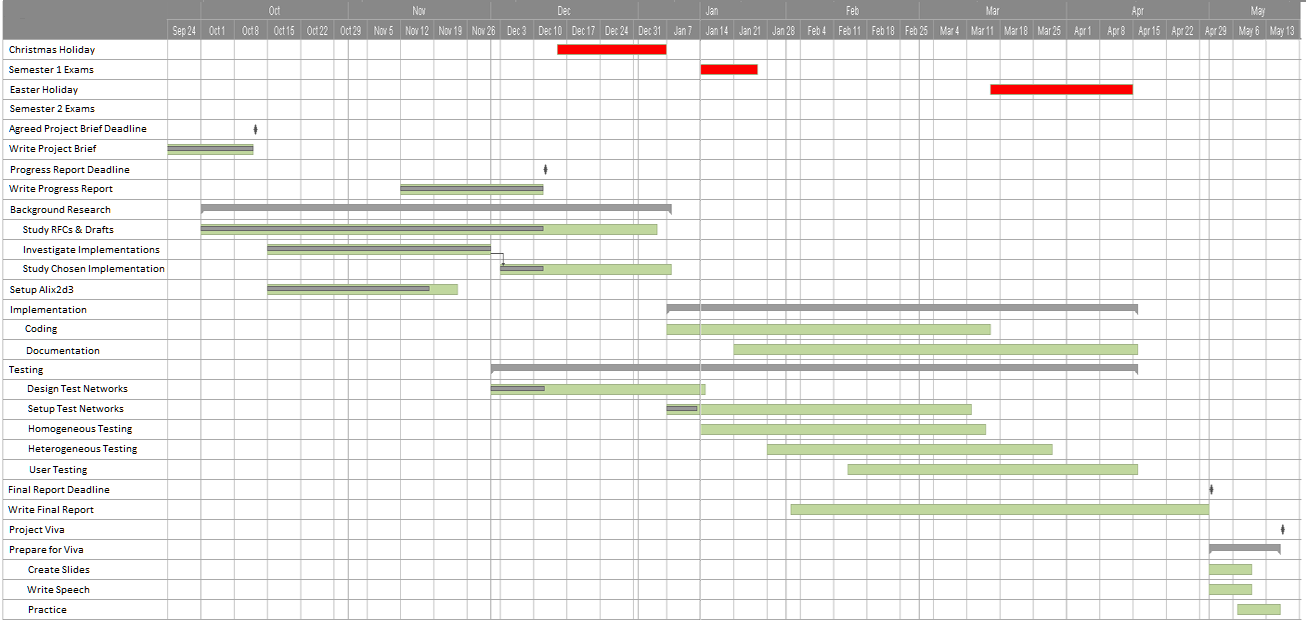
\includegraphics[width=1.\linewidth]{../Gantt/EvenBetterDec.png}
\end{center}

\pagebreak

\subsection{Final Gantt Chart}
This Gantt chart shows how my project actually progressed.

\begin{center}
  \hspace*{-0.75cm}
  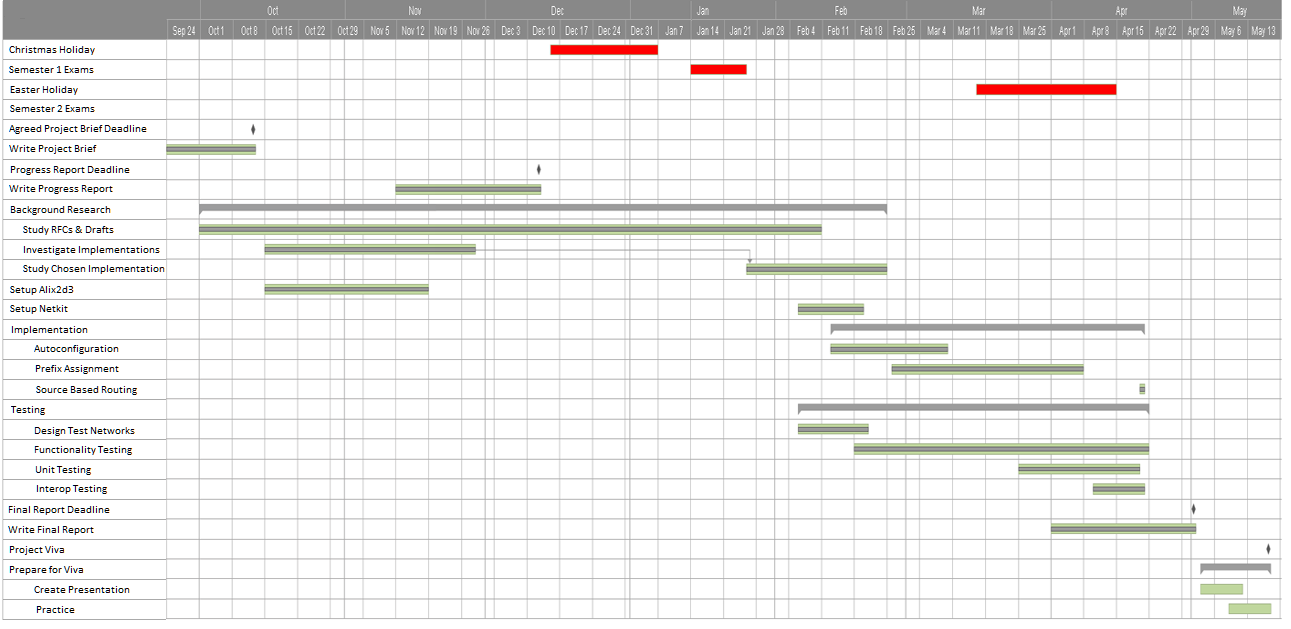
\includegraphics[width=1.\linewidth]{../Gantt/EvenBetterApril.png}
\end{center}

\end{landscape}

\pagebreak

\chapter{Evaluation}

\section{What Went Well?}
In general the project was a success. Despite its difficulty, I managed to
complete my implementation on schedule. I feel the software I have produced is
functional, robust and maintainable. I managed to meet all my goals, and the
only requirement that I did not fulfil was number 8: obtaining aggregated
prefixes from DHCP-PD\@. My code is now ready for code review, after which it may
be accepted as part of Quagga. The feedback on the drafts I produced should
help them progress along the standards track.

I enjoyed working in a language and style of programming with which I had
little experience -- I have learnt a huge amount about how procedural
programming differs from an object oriented approach. My C programming ability
has improved dramatically, and I have a much better understanding of pointers
and \texttt{struct}s, and in turn, the low-level operation of computers.  

I am now more confident working on large projects. Before this project, I
looked at open source code bases and felt intimidated by their size and style.
I was unsure where the code for these applications even began executing.
Having completed this project, I realise that the statements making up large
projects are no different from ones I am familiar with from my own work --
there is rarely anything that when taken in isolation, I am unable to
understand.

I learnt a lot about software projects that exist to support networking.
Not only did I discover Quagga, but I also learnt about many other projects. I
used competing routing daemon implementations: Bird and XORP\@. I also read
about Cisco's proprietary implementations of these protocols. I made heavy use of
\texttt{iproute2}, the package that has superseded \texttt{ifconfig} as the de
facto way to control TCP/IP networking in Linux. I also experimented with
\texttt{radvd} the Router Advertisement Daemon, and played with WIDE-DHCPv6. 

\section{What Could Have Gone Better?}
Although the project generally went well, perfection is rarely obtainable, and
there are things that if I did this project again, I would do differently. 

Firstly, due a high workload from other modules at the end of Semester One, I
did not dig into the project until later than I would have liked -- in
hindsight I could have chosen less coursework intensive optional modules.
Another factor was my lack of confidence about jumping in at the deep end.
Working on this project taught me that one of the best ways of understanding
a code base is trying adding a feature to it.

I also feel that I could have become more involved in the discussion about the
drafts, again I think I was held back by a lack of experience and confidence,
having never been involved with the Internet Engineering Task Force or any
other international standards body before. 


\chapter{Conclusions and Future Work}

\section{Conclusions}
In this project I have shown that it is possible to extend Quagga to implement
zero configuration OSPFv3; Along the way I learned a lot about networks. 

\subsection{Ambiguities in the Drafts}
There are a few areas of the drafts that I feel are slightly ambiguous or under
prescriptive. I plan on sending the following suggestions to the authors of the
drafts.

The following comments refer to the Autoconfiguration draft
\cite{draft-ietf-ospf-ospfv3-autoconfig-02}:
\begin{enumerate}
	\item In section 5.1 the draft says: 
		%\begin{quote}

		``An OSPFv3 router implementing this specification should assure that the
		inadvertent connection of multiple router interfaces to the same physical
		link in not misconstrued as detection of a different OSPFv3 router with a
		duplicate Router-ID.'' 
		%\end{quote}

		 I feel the draft should be more prescriptive on this issue.  My
		 implementation checks the router's interfaces link local addresses,
		 comparing them to the source address of the packet, I am not sure this is
		 correct.
	\item Section 7 states:
		%\begin{quote}

		``It is RECOMMENDED that OSPFv3 routers supporting this specification
		also allow explicit configuration of OSPFv3 parameters as specified
		in Appendix C of [OSPFV3].''
		%\end{quote}

		It does not mention what to do upon a conflict between an automatically
		generated and a manually configured Router-ID: The two routers decide
		independently whether they will change. If the autoconfigured router
		determines that the other must change its RID, we will be left in a
		conflicting state.
	\item  The non-neighbour case (5.2) for RID collisions covers all collisions,
		it should cover the neighbour case (5.1). A justification for the existence
		of the neighbour case might be beneficial.
\end{enumerate}

These suggestions are about the prefix assignment draft
\cite{draft-arkko-homenet-prefix-assignment-03}:
\begin{enumerate}
	\item Section 8 says:
		%\begin{quote}

		``A new prefix assignment within an aggregated prefix SHOULD NOT be
		committed before the router has waited NEW\_PREFIX\_ASSIGNMENT seconds for
		another prefix or reachable OSPFv3 router to appear.''
		%\end{quote}

		The draft doesn't state exactly what is meant by committed. As mentioned in
		Section~\ref{pending_list}, I used a pending list to ensure a young
		conflicting assignment could be deleted quickly.
	\item The draft does not indicate how assignments should be chosen. Using a
		random or sequential value seems obvious, but it may be possible to reduce
		routing table entries by employing a scheme that facilitates route
		aggregation. 
\end{enumerate}

\section{Continuing the project}
Now the project is over, I plan to continue working on my implementation. My
goal is to have my code merged back into the Quagga mainline. Before this can
happen, the code will need to go through a cleanup stage and a series of code
reviews to ensure it is of sufficient quality, and fits well with the Quagga
project.

This summer I hope to attend the 87th IETF meeting, I have been awarded
the ECS Student Development fund to help fund the trip. Attending this event
will give me the opportunity to discuss future work, and participate in
interoperability tests.

\section{Future Work}
My project had a large scope, is in a topical research area, and is based on
highly extensible drafts. As such a large amount of work can be based on what I
have produced. 

This project is a good candidate for extension by a Google Summer of Code
student, or a future Third Year Project. 

\subsection{DHCPv6-PD}
Ideally an implementation of OSPFv3 Prefix Assignment should handle aggregated
prefixes delegated by DHCPv6-PD\@. I decided early on in the project that this
was beyond the scope of the project. 

There are two ways I would suggest implementing this functionality. The first
is to make use of an existing DHCPv6 Client such as WIDE-DHCPv6, and hook into
its PD message functionality. The other would be to add functionality to Quagga
itself to handle the DHCPv6-PD messages. 

I feel implementing this as part of Quagga is the better solution as it does
not couple Quagga to other projects. However, it would be likely to require
more work to achieve.

\subsection{Source Based Routing} 
My proof-of-concept code (See Section~\ref{SourceBasedRouting}) shows that it
is possible to do source based routing by extending Quagga. A more formal
implementation of source based routing would be beneficial to the community.
Ideally it would conform to the drafts, and be consistent with Quagga's
existing coding style. 

\subsection{Multi-hop Service discovery}
Service discovery is very popular in modern networks. Major use cases include
finding media streamers and printers on a home network. At present, since the
service discovery messages are not forwarded by the router, to discover a
service, a host must be on the same subnet.

It would be possible to extend Quagga to flood service discovery
messages across the whole network, enabling services on one subnet, to be
discoverable from another. Uses for this include: monitoring home appliances from
within the home workstation network, and displaying images on a public screen
from a guest network.

There are currently no drafts indicating how to do this. Ideally Apple Inc.\@
would extend their service discovery platform, Bonjour, to use this kind of
technology.

\subsection{Domain Name Services}
In a typical single subnet IPv4 home network, DNS servers  are learned through
DHCP from an ISP, or manually configured. In a multi-subnet home network,
mechanisms are needed for propagating the DNS severs available to the network.
The prefix assignment draft recommends supporting stateless DHCPv6 and Router
Advertisement options.

Stateless DHCPv6 works by running a DHCPv6 server that maintains no state about
its clients. It simply serves configuration details such as the DNS server
addresses. The draft recommends that each router acts as a DHCPv6 relay so
hosts deep within the network can obtain DNS information.  Enabling DHCPv6
should be simple as packages (Such as WIDE-DHCPv6, Dibbler) already exist. 

Router advertisements contain two types of listing for discovering DNS servers.
First, listings for Recursive DNS Servers (RDNSS)
\nomenclature{RDNSS}{Recursive DNS Server}: Servers that will recursively
resolve Domain Names. Secondly, DNS Search Lists (DNSSL)
\nomenclature{DNSSL}{DNS Search List}, a list of servers that can be used to
resolve local names. Adding this functionality to my implementation would be
more difficult that adding stateless DHCPv6 as Quaggas Router advertisement
code would need to be modified to deal with these options.

The draft does not mention whether configuration learned through either method
should be consolidated, and advertised through both. If this is required,
complexity would increase.

\subsection{Security Considerations} 
Built in security was a feature of OSPFv2 but was removed in OSPFv3 in favour
IPSec (IP Security). IPSec is difficult to deploy so is not suitable for home
users. RFC6506 reintroduces OSPF security through the use of an Authentication
Trailer\cite{rfc6506}. Implementing this RFC would add Security to
Autoconfigured networks. Users would need to choose a secret key and enable
authentication trailers to prevent unauthorised routers joining their home
network.  

\section{Deployment in the Home}
As IPv6 becomes more common place, and IPv4 is slowly phased out, this project can 
actually be used in the home. For home users to want to switch to IPv6 there must 
be features they cannot get from IPv4 -- I feel that this project 
implements one of those features.

It does not however stop at home users, ISPs also need to be on board.
Currently in the UK there is only a handful of ISPs providing IPv6 addresses to
their customers. SixXS list just seven UK ISPs, the most popular of these being
Andrews \& Arnold \cite{SixXS}.

These problems are outside of my control, hopefully with time, the
large ISPs will overcome the inertia of switching to IPv6.

\raggedbottom
\pagebreak

\phantomsection
\printnomenclature
\addcontentsline{toc}{chapter}{Nomenclature}
\raggedbottom
\pagebreak

\phantomsection
\addcontentsline{toc}{chapter}{Bibliography}
\bibliography{FinalReport}{}
\bibliographystyle{ieeetr}

\appendix 
%\appendixpage

\begin{landscape}
\chapter{Typical Home Networks}
\section{Present}
\label{typical_homenet_present}
\begin{center}
	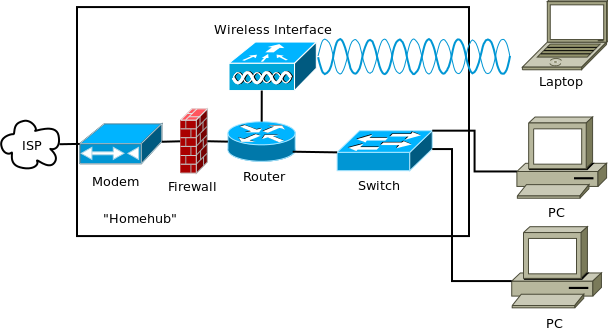
\includegraphics[width=0.75\linewidth]{../Diagrams/Network/TypicalHomenet.png}
\end{center}
This diagram shows a typical home network in the present day. The hardware
inside the box labeled ``Homehub'' is typically provided to customers as one
plug in and play device. It is commonly referred to as a router, although this
is slightly misleading as they perform many other tasks that routing.

As can be seen from the diagram, the box provides the house with wired and
wireless connections to the LAN and the internet. The WLAN is typically bridged
with the LAN to give create a single subnet.

\section{Future}
\label{typical_homenet_future}
\begin{center}
	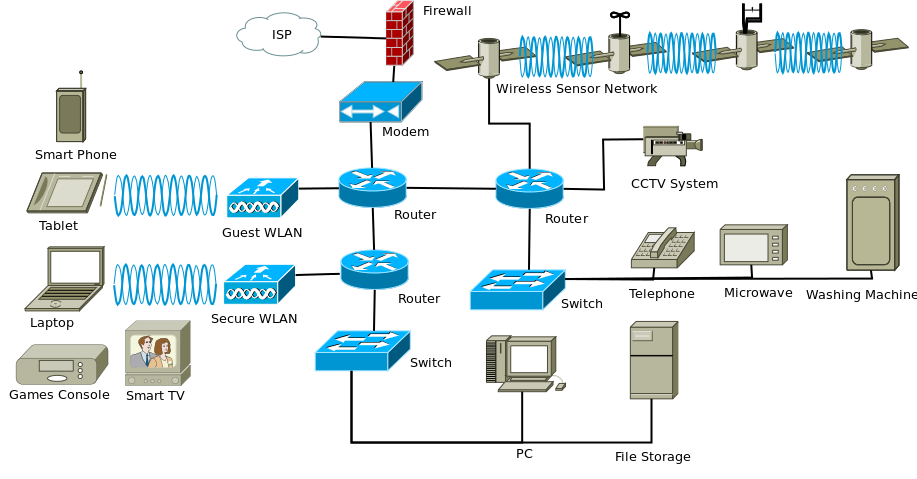
\includegraphics[width=0.9\linewidth]{../Diagrams/Network/FutureHomenet.png}
\end{center}
This diagram shows a hypothetical future home network. The network includes a
guest wireless network, a secured wireless network, a wired network, a network
for appliances, a network for a home surveillance system and a wireless sensor
network.

\chapter{Typical Corporate Network}
\label{typical_corporate_net}
\begin{center}
	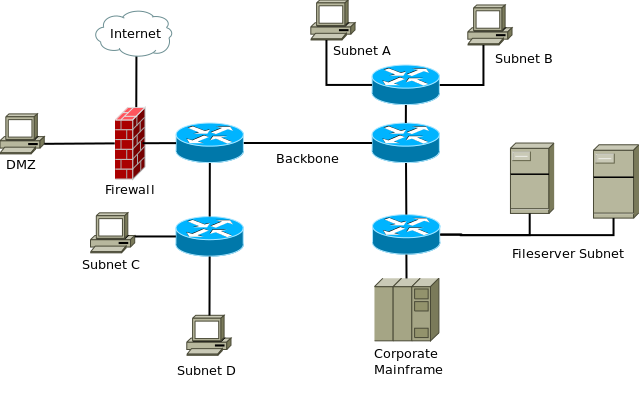
\includegraphics[width=0.75\linewidth]{../Diagrams/Network/CorporateNetwork.png}
\end{center}
This diagram shows the typical topology of a corporate network. For the sake of reducing complexity, Layer 2 switches have not been shown.

\end{landscape}

\chapter{Packets}
Images created with http://interactive.blockdiag.com/packetdiag/

\section{Auto Configuration LSA}
\label{AC-LSA}
\begin{center}
	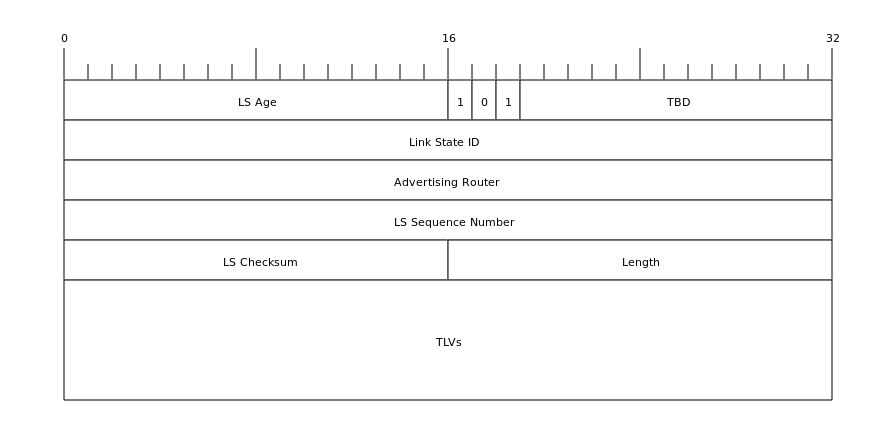
\includegraphics[width=\linewidth]{../Diagrams/Packets/ac_lsa.png}
\end{center}

\section{TLV}
\label{TLV}
\begin{center}
	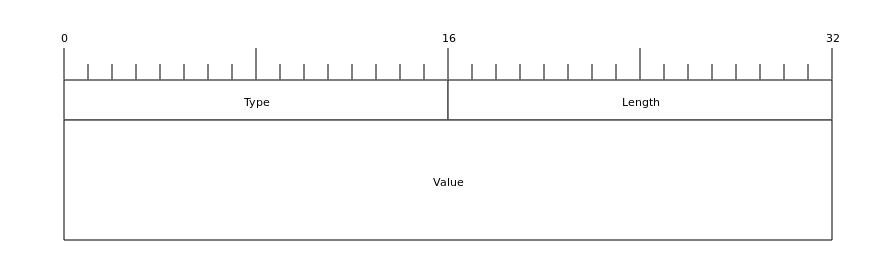
\includegraphics[width=\linewidth]{../Diagrams/Packets/tlv.png}
\end{center}

\section{Router Hardware Fingerprint TLV}
\begin{center}
	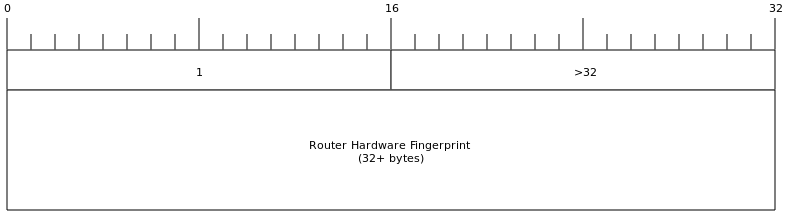
\includegraphics[width=\linewidth]{../Diagrams/Packets/rhwfp_tlv.png}
\end{center}

\section{Aggregated Prefix TLV}
\begin{center}
	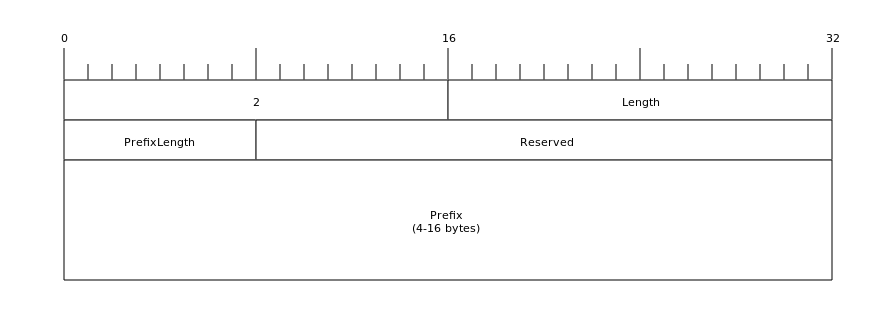
\includegraphics[width=\linewidth]{../Diagrams/Packets/aggregated_prefix_tlv.png}
\end{center}

\section{Assigned Prefix TLV}
\begin{center}
	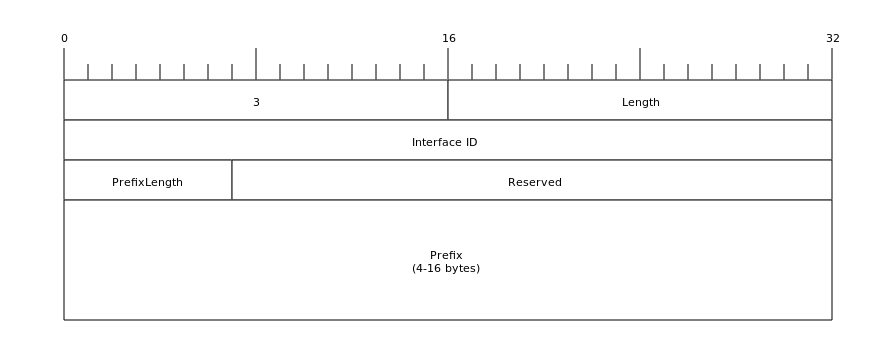
\includegraphics[width=\linewidth]{../Diagrams/Packets/assigned_prefix_tlv.png}
\end{center}

\chapter{Netkit Test Networks}

\section{Simple Network}
\begin{center}
	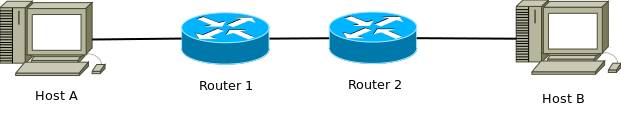
\includegraphics[width=\linewidth]{../Diagrams/Network/SimpleNetkit.png}
\end{center}

\section{Main Network}
\begin{center}
	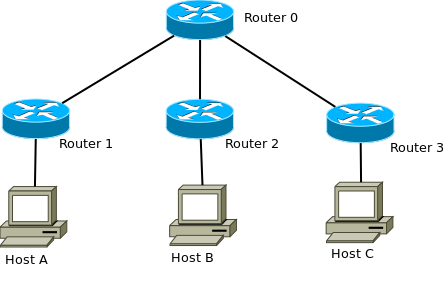
\includegraphics[width=\linewidth]{../Diagrams/Network/MainNetkit.png}
\end{center}

\chapter{Github Stats}
\label{GithubStats}

\section{Github Commit Graph}
\begin{center}
	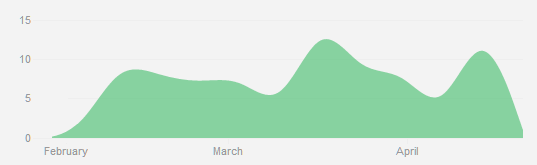
\includegraphics[width=\linewidth]{../Diagrams/Stats/GitHubCommitGraph.png}
\end{center}

\section{Github Punchcard}
\begin{center}
	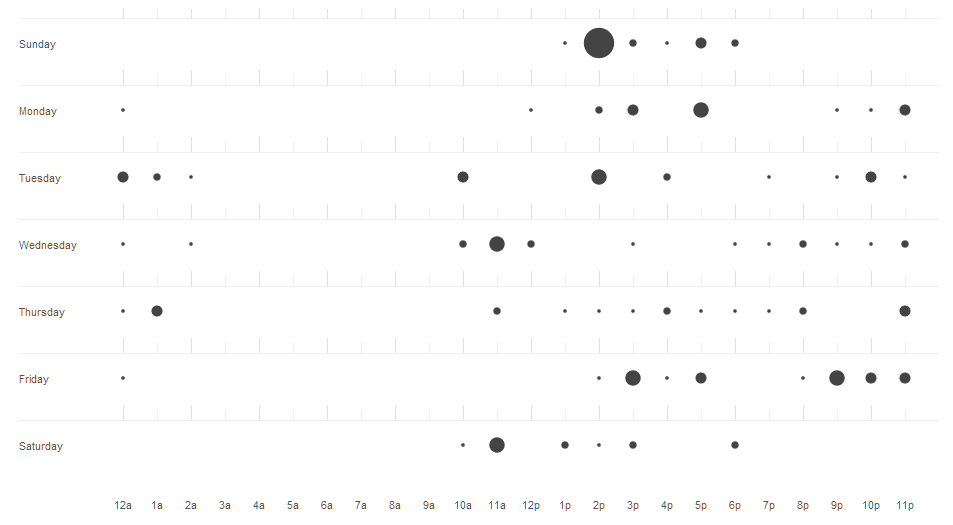
\includegraphics[width=\linewidth]{../Diagrams/Stats/GitHubPunchCard.png}
\end{center}

\chapter{Alix2d3}
As the project progressed it became clear that they Alix2d3s were not as useful
as was originaly believed, thanks to discovery of the briliant software package
Netkit. I did however undertake testing on the Alix2d3s. If someone wished to
repeat my experimentation, the following guides would be helpful. 

\section{Installation Guide}

 This guide\cite{germanGuide} offered a comprehensive list of steps that need to
 be taken to install Ubuntu Linux on a PC Engines alix2d3\cite{alix2d3}.  The article is
 written in German but using Google translate I was able to follow it as it is
 mainly a list of shell commands.

 The process begins with installing the compact flash card as a device on an
 existing Ubuntu desktop PC\@. Next the card is partitioned using \texttt{fdisk},
 the card is then formatted as ext2 (a Linux file system type) using
 \texttt{mk2fs}. The card is then mounted in the file system, using
 \texttt{mount} and a small installation of Linux is copied to the card using
 \texttt{debootstrap} to provide a base system.

 Several settings and devices are linked to the flash cards mount point and
 \texttt{chroot} is used to simulate booting into the new install. The required
 configuration files are edited (e.g.\@ network interface settings) and essential
 software packages (such as \texttt{Vim}, \texttt{SSH}, \texttt{sudo}, and
 \texttt{APT}) are installed. A boot loader such as \texttt{GRUB} is also
 installed and configured.

 Next, the flash card is safely removed, and  inserted into the alix2d3. The
 alix2d3 is then powered on. Using a USB to Null Model cable connecting a PC to
 the alix2d3's serial port, a terminal connection can be established using {\bf
 cu}. I had a few problems using this device (\texttt{ttyUSB0}) but I was able to
 fix this problem using \texttt{chown}. This terminal connection can be used to
 aid the boot process and ensure that there are no Magic ELF errors. Once the
 alix2d3 is up and running it is possible to disconnect the serial cable and
 access it over \texttt{SSH} alone.

 \section{Quagga Installation Guide}

 \subsection{Normal Installation}
This is a procedure that has  turned out to be far more difficult that anticipated.

First of all, need to ensure that all the dependencies are present. The easiest
way I have found to do this is to use:

sudo apt-get build-dep quagga

This should fetch all the packages that quagga depends on. I see no reason to
build these from source, since I shall not be modifying them.

It seems that a package called libtool is also needed to ensure installation works.
Not certain this is needed.

\ libreadline also seems to be an issue (mainly with vtysh):

\texttt{sudo apt-get install lib32readline6}

Next it should be possible to run \texttt{\@./bootstrap}. As far as I know this
produces (among other things) the configure script.

Next run the configure script. This [wiki][wiki] suggests that it is best to
move the folders using:

\texttt{sudo \@./configure --sysconfdir=/usr/local/quagga --localstatedir=/usr/local/quagga}

The configure script will prompt you to create a user called quagga. Do this by:

sudo adduser quagga
sudo mkdir /usr/local/quagga
sudo chown quagga:quagga /usr/local/quagga

It is now time to run make. See the crosscompiling document for more
information about this. Previously I had issues with zebra making, to fix this
manually editing the Makefile in \@./zebra by adding -lcap to LIBS\@. This doesn't
seem to be a problem with the latest source.

Run sudo make install. This should install everything, and the daemons
should have installed themselves to /usr/local/sbin.

Now a little bit of configuration is required. \texttt{cd /usr/local/quagga}.
Either make a real config file for the daemon, or just create a file containing ``password test''.


You should now be able to run sudo ospf6d. If you can't, try ldconfig.


[wiki]: http://wiki.nil.com/Installing\_and\_running\_Quagga

\subsection{Cross Compilation}

Since Alix2d3s are very slow, a build of Quagga can be incredibly slow. The make parts
alone can take around 15 minutes. (I actually found that XORP had an even slower
compile time, in the order of hours) 

To over come this issue it is possible to compile the source code on a much
faster machine (e.g.\@ desktop pc) and copy it across. 

Since modern machines use a 64bit architecture rather than 32bit like the
Alix2d3s, the compiler must be set up correctly. Adding the cflag ``-m32'' should
suffice, however to be on the safe side, ``-m32 -march=i386'' can be used. 

This should be done by appending '--with-clfags=``-m32 -march=i386i''' to \@./configure.

I initially had problems with this compilation. I resolved the issues by going
back to basics and trying to compile a simple helloworld program for the Alix.
Turns out I was missing ``gcc-multilib''. This can be installed with apt.

\chapter{vtysh}
\label{vtysh}

Commands are added using DEFUN and install.

I added the commands:
\begin{itemize}
  \item show ipv6 ospf6 prefix aggregated
  \item show ipv6 ospf6 prefix allocated 
  \item show ipv6 ospf6 prefix assigned X

  \item enable $>$ configure terminal $>$ ipv6 allocate-prefix X:X::X:X/M
  \item enable $>$ configure terminal $>$ no ipv6 allocate-prefix X:X::X:X/M
\end{itemize}


\end{document}
